%
% Tallinn University of Technology - bachelor, master thesis template for LaTeX
%
% Public version 1.2
% 2022 Updated by Karl Janson to match the new formatting guidelines
%
% Public Version 1.1
% 2019 Adjusted by Frank Korving for his Bachelor Thesis, with contributions from Sander Arnus
%
% Public version 1.0
% 2010 - 2013 Thijs Nugteren and Joos Buijs for Master Thesis
%
% THIS IS THE MAIN FILE (i.e. compile this file, compiling the others directly won't work)
%

\documentclass[12pt, a4paper]{report}

% all the other includes etc. are done in the thesis.sty file.
\usepackage{thesis}
\usepackage{ifthen}
\usepackage{datetime}

\renewcommand{\dateseparator}{.}

%%%%%%%%%%%%%%%%%%%%%%%%%%%%%%%%%%%%%%%%%%%%%%%%%%%%%%%%%%%%%
% NOTE:                                                     %
%%%%%%%%%%%%%%%%%%%%%%%%%%%%%%%%%%%%%%%%%%%%%%%%%%%%%%%%%%%%%
% * Content chapter files are located in "chapters" folder, %
%   included using the "chapters_main.tex" file             %
%                                                           %
% * Appendices are located in "appendices" folder,          %
%   included using the "appendices_main.tex" file           %
%%%%%%%%%%%%%%%%%%%%%%%%%%%%%%%%%%%%%%%%%%%%%%%%%%%%%%%%%%%%%

%%%%%%%%%%%%%%%%%%%%%%%%%%%%%%%%%%%%%%%%%%%%%%%%%%%%%%%%%%%%%
% The commands below need to be defined.                    %
% Estonian title page will be generated automatically       %
%%%%%%%%%%%%%%%%%%%%%%%%%%%%%%%%%%%%%%%%%%%%%%%%%%%%%%%%%%%%%
\newcommand{\doctitle}{Stateful Stream Processing: A Comparative Analysis of Apache Flink and Kafka Streams frameworks}
\newcommand{\doctitleEst}{Olekupõhine voogtöötlus: Apache Flink ja Kafka Streams raamistike voogtöötluse võrdlus} % Title in Estonian

% Choose one
\newcommand{\doctype}{Master's Thesis}

% Thesis author
\newcommand{\authorName}{Aleksandr Madisson}
\newcommand{\studentcode}{221249IAPM}

% Main supervisor
\newcommand{\supervisor}{Radu Irbe}
\newcommand{\supervisortitle}{M.Sc.}

% Co-supervisor. If you have only one supervisor, leave it as it is
\newcommand{\cosupervisor}{[Co-Supervisor's Name]}
\newcommand{\cosupervisortitle}{[Academic degree]}

% Dates. Default to current current date. 
% You can hard code a value by replacing the parameter with a text
% Year of publication (defaults to current year).
\newcommand{\Year}{\the\year{}}

% Signature date (defaults to today).
\newcommand{\signatureDate}{\ddmmyyyydate\today}

% PDF Metadata
\newcommand{\version}{0.1 version}
\newcommand{\keywords}{Important, comma, separated, keywords, applicable, to, your, thesis}

%%%%%%%%%%%%%%%%%%%%%%%%%%%%%%%%%%%%%%%%%%%%%%%%%%%%%%%%%%%%%
%            DO NOT EDIT BELOW THIS LINE                    %
%%%%%%%%%%%%%%%%%%%%%%%%%%%%%%%%%%%%%%%%%%%%%%%%%%%%%%%%%%%%%

\newcommand{\university}{TALLINN UNIVERSITY OF TECHNOLOGY}
\newcommand{\school}{School of Information Technologies}
\newcommand{\universityEst}{TALLINNA TEHNIKAÜLIKOOL}
\newcommand{\schoolEst}{Infotehnoloogia teaduskond}

% For Estonian title page generation
\newcommand{\meEst}[1]
{
  \ifthenelse{\equal{#1}{[Author name]}}{[Ees- ja perenimi]}{\authorName}
}

\newcommand{\studentcodeEst}[1]
{
  \ifthenelse{\equal{#1}{[Student Code]}}{[Üliõpilaskood]}{\studentcode}
}

\newcommand{\doctypeEst}[1]
{
  \ifthenelse{\equal{#1}{[Bachelor's Thesis / Master's Thesis]}}{[Bakalaureusetöö / Magistritöö]}{}
  \ifthenelse{\equal{#1}{Bachelor's Thesis}}{Bakalaureusetöö}{}
  \ifthenelse{\equal{#1}{Master's Thesis}}{Magistritöö}{}
}

\newcommand{\supervisorEst}[1]
{
  \ifthenelse{\equal{#1}{[Supervisor's Name]}}{[Juhendaja nimi]}{\supervisor}
}
\newcommand{\supervisortitleEst}[1]
{
  \ifthenelse{\equal{#1}{[Academic degree]}}{[Teaduskraad]}{\supervisortitle}
}

%
% PDF settings
%
\hypersetup
{
    pdfauthor={\authorName},
    pdfsubject={\doctitle},
    pdfkeywords={\keywords}
}

\begin{document}

% Pages like title, auhtor's declaration, etc.
% ENGLISH TITLE PAGE

\begin{titlepage}
\headheight = 57pt
\footskip = 5pt
\headsep = 0pt

\centering
\university\\
\school

\vspace*{4.5 cm}

\begin{center}

\authorName~~\studentcode\\
\vspace*{1.5 cm}

\begin{Large}
\textsc{\textbf{\doctitle}}\\
\end{Large}

\vspace*{1.5 cm}
\doctype\\
\end{center}

\vspace*{0.6 cm}

\begin{flushright}
Supervisor: \supervisor\\\supervisortitle\\
\vspace*{0.2 cm}

\ifthenelse{\equal{\cosupervisor}{[Co-Supervisor's Name]}}{}{Co-supervisor: \cosupervisor\\\cosupervisortitle}
\end{flushright}
\vfill

Tallinn \Year
\end{titlepage}

\pagebreak

% ESTONIAN TITLE PAGE
%\begin{titlepage}
%\headheight = 57pt
%\footskip = 5pt
%\headsep = 0pt
%
%\centering
%\universityEst\\
%\schoolEst
%
%\vspace*{4.5 cm}
%
%\begin{center}
%
%\meEst{\authorName}\studentcodeEst{\studentcode}\\
%\vspace*{1.5 cm}
%
%\begin{Large}
%\textsc{\textbf{\doctitleEst}}\\
%\end{Large}
%
%\vspace*{1.5 cm}
%\doctypeEst{\doctype}\\
%\end{center}
%
%\vspace*{0.6 cm}
%
%\begin{flushright}
%Juhendaja: \supervisorEst{\supervisor}\\\supervisortitleEst{\supervisortitle}\\
%\vspace*{0.2 cm}
%\ifthenelse{\equal{\cosupervisor}{[Co-Supervisor's Name]}}{}{Kaasjuhendaja: \cosupervisor\\\cosupervisortitle}
%\end{flushright}
%\vfill
%
%Tallinn \Year
%\end{titlepage}

\setcounter{page}{0}
\pagenumbering{arabic}   %from here on, start the 'real' page numbering, from 1, with normal digits

\normalsize

\chapter*{\centerline{Author's Declaration of Originality}}\label{chapter:declaration}
I hereby certify that I am the sole author of this thesis. All the used materials, references
to the literature and the work of others have been referred to. This thesis has not been
presented for examination anywhere else.

% \vspace*{0.5cm}
\begin{flushleft}

Author:~\authorName\\
\vspace*{0.5cm}
\signatureDate
 
\end{flushleft}
\pagebreak

\chapter*{\centerline{Abstract}}\label{chapter:abstract}
Software engineering is a diverse field that focuses on addressing various business domain problems.
These domain-specific issues and their corresponding use cases necessitate in-depth analysis to determine
the most suitable technologies for achieving optimal problem-solving outcomes.
One rapidly growing area in software engineering is big data.
Although big data is sometimes regarded as a marketing term, it encompasses complex data processing frameworks and datasets.

As the volume of produced data has dramatically increased over the years,
modern technical solutions capable of processing massive amounts of data are required.
The open-source community offers a decent frameworks and tools, making it challenging to choose the best option.
This research focuses on comparing the most suitable frameworks for specific use cases,
particularly those that designed for stateful real-time stream processing.

Stream processing use cases are relatively rare compared to typical problems that can often
be solved with traditional batch processing or simple program which doesn't require MapReduce
model or DAG.
However, stateful stream processing assumes that real-time processing relies on previous states,
and unbounded data flow which may indicate abnormal system behavior, such as fraud alerts in financial transactions
within a specific time frame.
Quick response can facilitate necessary actions and save time.
Therefore, it is crucial to provide a technical analysis of the most suitable frameworks,
assess their advantages and disadvantages, and examine the complexities involved in their
application for stateful stream processing based on given use case.
This master's thesis offers a technical overview,
benchmarks, and comparisons for appropriate use cases.
The use case examines considers that each incoming event triggers state re-computation and
evaluates how efficiently Kafka Streams and Apache Flink manage state under heavy loads,
represented by a stream of Kafka messages.
The ideal framework should address existing problems while offering excellent scalability,
fault tolerance, and cost efficiency.
This master's thesis aims to provide an answer and a technical overview based on the given requirements.
\pagebreak

%\chapter*{\begin{center}Annotatsioon\\\large\doctitleEst\end{center}}\label{chapter:abstract-eesti}
%[YOUR TEXT GOES HERE]

Lõputöö on kirjutatud [mis keeles] keeles ning sisaldab teksti [lehekülgede arv] leheküljel, [peatükkide arv] peatükki, [jooniste arv] joonist, [tabelite arv] tabelit.
%\pagebreak

\chapter*{\centerline{List of Abbreviations and Terms}}\label{chapter:terms}
\begin{longtable}{p{3cm}p{10cm}}
    EKS  & Elastic Kubernetes Service         \\
    ECR  & Elastic Container Registry         \\
    EC2  & Amazon Elastic Computer Cloud      \\
    MSK  & Amazon Managed Streaming           \\
    AWS  & Amazon Web Services                \\
    HA   & High Availability                  \\
    YARN & Yet Another Resource Manager       \\
    DAG  & Directed Acyclic Graph             \\
    JVM  & Java Virtual Machine               \\
    K8S  & Kubernetes                         \\
    MP   & MapReduce                          \\
    TB   & Terabyte                           \\
    UC   & Use Case                           \\
    JMX  & Java Management Extension          \\
    API  & Application Programming Interface  \\
    CPU  & Central Processing Unit            \\
    IDE  & Integrated Development Environment \\
    IOT  & Internet Of Things                 \\
    VM   & Virtual Machine                    \\
    EBS  & Elastic Block Store                \\
\end{longtable}
\addtocounter{table}{-1} 
\pagebreak

\phantomsection
\setcounter{tocdepth}{2}    % Sets maximum depth of Table Of Contents
\renewcommand{\contentsname}{Table of Contents}
\tableofcontents

\clearpage \phantomsection
\setcounter{figure}{0}
% \addcontentsline{toc}{chapter}{\listfigurename}
\listoffigures

\clearpage \phantomsection
% \addcontentsline{toc}{chapter}{\listtablename}
\listoftables


% Content chapters
\chapter{Introduction}\label{ch:introduction}
%Some basic ways to manipulate text are \textit{italics} and \textbf{bold}. One can reference Figures (see Figure \ref{fig:taltech} for an example) as well as cite references which are defined in the \textit{references.bib} file.\cite{spectre,example-reference}
%
%The \textit{Bibliography}, \textit{List of Figures} and \textit{List of Tables} are all automatically generated and references will be updated automatically as well. This means that if you've defined a citation but are not referencing it, it will not appear in the \textit{Bibliography}. This also means that any Figure / Table / Citations numbers are automatically updated as well. Numbering is done by order-of-appearance.
%
%One can create an itemized list:
%\begin{itemize}
%    \item item a
%    \item item b
%    \item ...
%\end{itemize}
%
%Or enumerate them:
%\begin{enumerate}
%    \item item x
%    \item item y
%    \item ...
%\end{enumerate}
%
%
%\begin{figure}[ht]
%    \centering
%    
\includegraphics[width=.5\textwidth]{figures/taltech.jpg}
%    \caption{\textit{An image of the TalTech logo.}}
%    \label{fig:taltech}
%\end{figure}
%
%
%A table with three columns can be seen in Table \ref{tab:requirements}.
%\begin{longtable}{|p{0,5cm}|p{10cm}|p{3cm}|}
%	\caption{\it{A table with some requirements}}
%	\label{tab:requirements}\\ \hline
%	\textbf{Nr} &  \textbf{Requirement} & \textbf{Weight}  \\
%	\hline
%	\endfirsthead
%	\multicolumn{3}{l}%
%	{\tablename\ \thetable\ -- \textit{Continues...}} \\ q
%	\hline
%	\textbf{Nr} &  \textbf{Requirement} & \textbf{Importance}  \\
%	\hline
%	\endhead
%	\hline \multicolumn{3}{l}{\textit{Continues...}} \\
%	\endfoot
%	\hline
%	\endlastfoot
%1 & Price & High\\ \hline
%2 & Variety& Middle\\ \hline
%3 & Support& Low\\ \hline
%
%\end{longtable}
%
%We can use variables set in the \textit{main.tex} file to render values like our title (\doctitle) or supervisor names (\textbf{Supervisor}: \supervisor, \textbf{Co-supervisor}: \cosupervisor{}).
%\section{What is a stream processing}\label{sec:stream-beg}
%Stream processing
%
%\section{Brief history of stream processing systems}\label{sec:breif-history}
%Stream processing


\section{Background and motivation}\label{sec:back-and-motiv}
A necessity in choosing the best suitable technology stack and a framework is
coming from a rapid growth of different kind of data sources which produce
a large volumes of data in a real time.
A definition of big data volumes has changed over time, and it's only growing.
The use case which is considered in this research is supposed to work with a
1TB of data per day, and it's obviously that in some time, for example, in
a couple of years 1TB might be won't be sufficient.
Another perspective of the first is to get an overview of open sources solutions
which could be successfully applied for appropriate use case.
Writing a custom big data framework would require too much effort,
and there's no guarantee that it will reach the same performance.
Obviously, if such framework could be written in assembly language,
which provide the best performance it wouldn't be possible to integrate
to a java based technology stack.
Fortunately, an open source community has grown a lot over the last years
and provides grate tooling for many use cases.
Considering open source solutions for a big data.

\newpage
\section{Problem statement}\label{sec:prob-st}
The problem is coming with a business demands which are based on a current needs
for a more scalable and efficient solution.
Before getting into a problem details, the current model will be provided, to
get better understanding why this research brings value and how streaming frameworks
are comparable with the current model.

\subsection{Current model overview}\label{subsec:current-model}

\begin{figure}[ht]
    \centering
    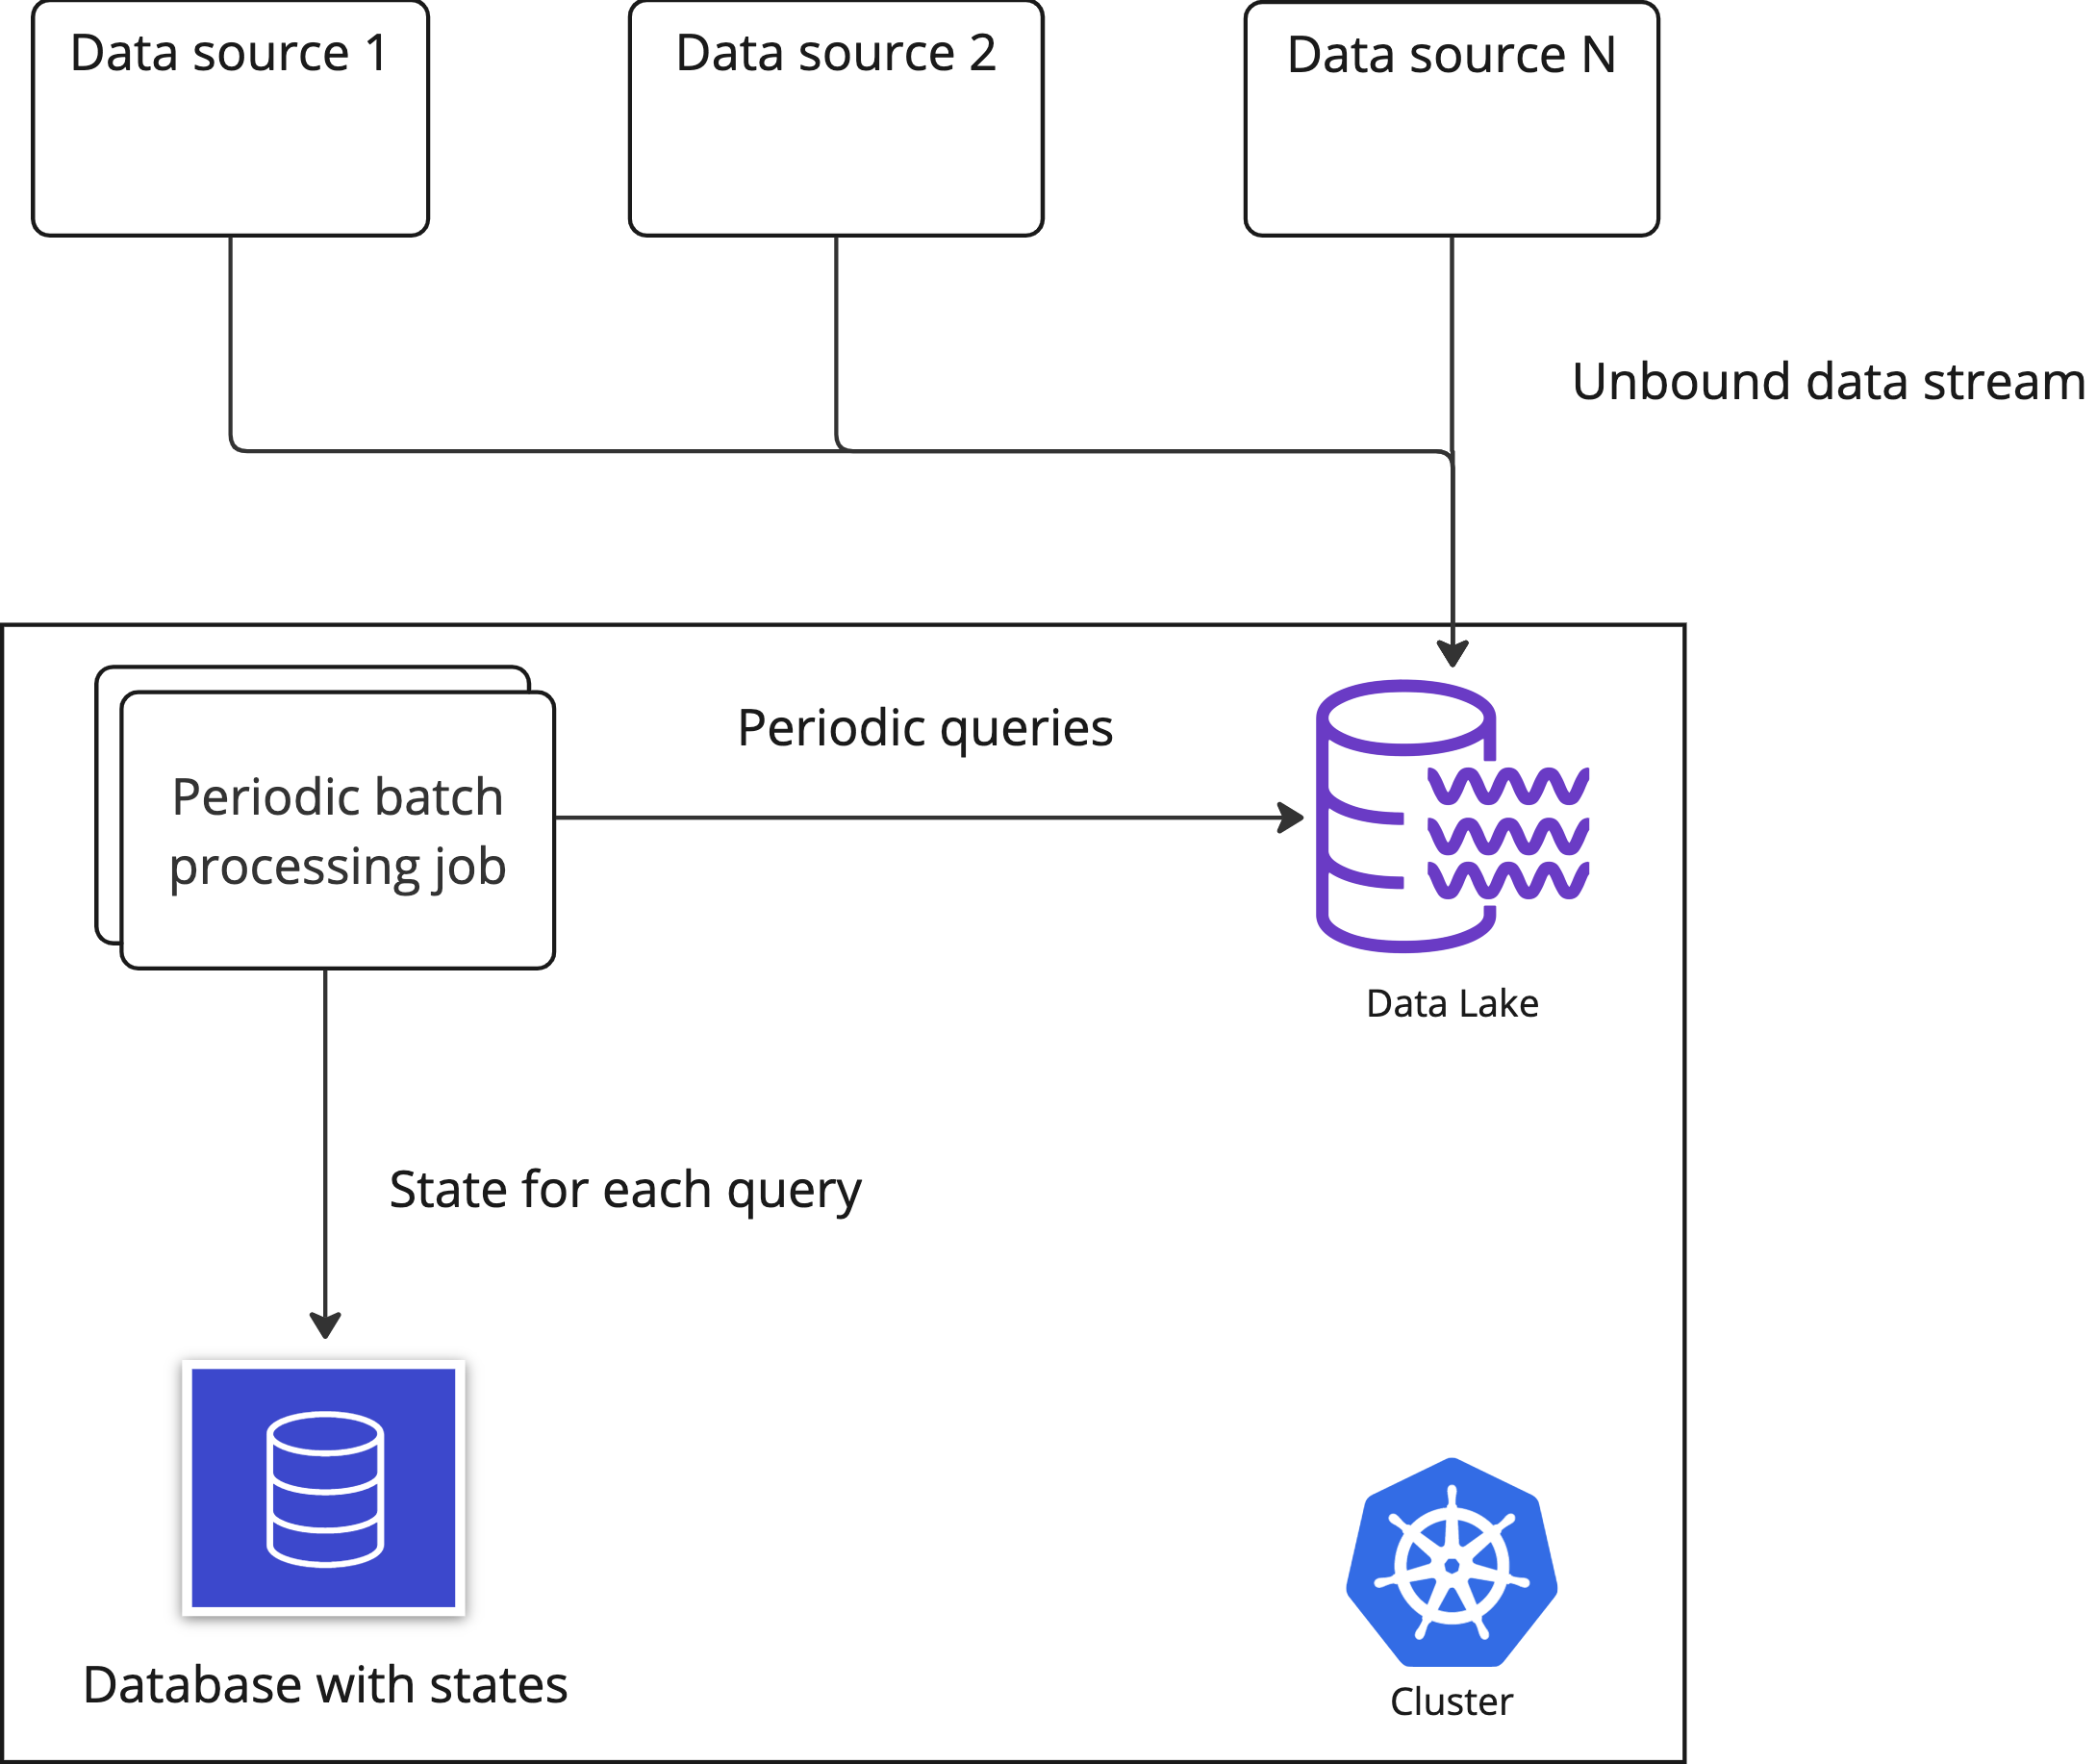
\includegraphics[width=.5\textwidth]{figures/current-model}
    \caption{\textit{Generic model of current data processing system.}}
    \label{fig:current-model}
\end{figure}

The figure\ref{fig:current-model} represents only a very generic model of the current
system to just get some overview.
The model contain the following components.

\begin{description}
    \item[Kubernetes cluster] An environment for cluster components.
    \item[Data course N] Is an external component which sends a data messages in unbound mode.
    Each data source is located in different external network and gets connected through
    a network gateway before it reaches the job.
    Each data messages gets saved in a data lake.
    \item[Processing job] Represents a functionality block which uses queries to access the
    data lake and save intermediate state to the state database.
    The job represents an application written in highly-level object-oriented programming language like Java, C\#
    and works in a batch processing mode which means it gets launched periodically.
    \item[Databse with states] Contains states for queries, a state is a crucial part of the job's pipeline.
    Contains an information from previous query executions.
    \item[Date late] Is a central data storage which provides a query interface.
\end{description}

From a first look, the system which is on the Figure \ref{fig:current-model} defines a straightforward
architecture.
Generally, the systems which implements such architecture are easily debuggable,
testable and quite often is a good way to go when the project gets started.
Everything might work smoothly for ages.
At some moment in time, the system might face with a breaking point which brings new challenges.

For example, in a few years, the number of data sources has significantly grown, where each
data source has its own sending frequency and a type.
A new load would require to add more and more instances of a job, faster period of job execution.
And also it leads to additional types of errors to handle, which haven't been seen before.
An execution of each query gets more expensive.
Not every data can be indexed, and especially if amount of indexed data has grown in many times, it adds
a significant complexity overhead for a query execution.
Moreover, additional errors might and circumstances may get the service down, which requires
additional balancing logic and a state recovery.
At might take a significant time to recover a service in specific region if this requires a manual work
from engineering team.

As a summary, some crucial problems can be defined as follows.

\begin{itemize}
    \item The system is not scalable enough.
    \item A state is lost after recovery, not completely fault tolerant.
    \item Expensive query execution, especially if data is not indexed
    \item Job processing is periodic, leads to a latency and limitation in processing time.
\end{itemize}

\newpage
\section{Research question and objectives}\label{sec:res-q-o}
Based on given description it's possible to set objectives and direction
where thesis research should be directed.
Obviously, that based on given major problems given as bullet points in previous section
some other sub problems appear which must considered in this research.

\subsection{Alternative architectures}\label{subsec:alternative-architectures-and-frameworks}
Fortunately, similar problems have already known in IT industry and big players like Google, Microsoft
have invested enough resources.
Their research results lead to a stream processing.
Stream processing is tend to be as alternative for bach processing which works for most cases, but
this specific use case if focused on real time data.
Once it's clear that stream processing is the way to go then comes a next question.
Another solution is to come up with a custom solution.
However, the most significant disadvantages include:

\begin{itemize}
    \item A need to hire a team just to developer another stream processing framework.
    \item There's a big change that a custom solution won't perform better than existing.
    \item Long-term engineering support, such as bug fixes, integration with external dependencies,
    feature development.
    \item The cost can become prohibitive.
\end{itemize}


At the same time, the open source community is huge enough, which supports the greatest
open source products under The Apache Software Foundation.
The most significant disadvantages include:

\begin{itemize}
    \item Industry standard frameworks.
    \item A huge support from developer around the world.
    \item An ease in extending already made code.
    \item Lots of ready for use tutorials and documentations.
    \item Many examples for different use cases.
\end{itemize}


\newpage
\subsection{Selecting a suitable framework}\label{subsec:selecting-a-suitable-framework}
They're lots different frameworks out there available for solving different
data streaming problems.
Most of the were born on top of each other as a new generation solution.
Each new framework is trying to bring better performance and scalability.
Down below is an evolution of streaming frameworks with a brief description:

\begin{description}
    \item[Apache S4 (2010)]  Apache S4 (Simple Scalable Streaming System) was an early stream
    processing engine developed at Yahoo! Labs.
    It was designed for unbounded data stream processing which uses
    simple programming model based on a publish/subscribe pattern.
    Apache S4 became an open source project under Apache Software Foundation but
    eventually became inactive due to limited community adoption.
    \item[Apache Storm (2011)]
    Apache Storm was a popular distributed stream processing framework.
    It was designed for real-time data processing and provided guarantees such as
    at-least-once and exactly-once processing semantics.
    Apache Storm was more popular comparing to Apache S4, but it provides less
    performance and flexibility comparing to next generation frameworks.
    \item[Apache Samza (2013)] Samza was developed at LinkedIn, as another distributed stream processing.
    Samza provided better integration for Kafka,
    offering strong durability guarantees and support for stateful stream processing.
    Samza also allowed users to perform windowed operations and join streams with external data stores.
    In general, Samza is a base for a next generation stream processing framework which called Kafka streams.
    \item[Apache Flink (2014)] Originally was developed at the Technical University of Berlin.
    Apache Flink is one of the most powerful stream processing framework that unified batch and
    stream processing with focusing on streaming.
    Flink provided low-latency, high-throughput, and exactly-once processing semantics.
    With its advanced features, such as event time processing, watermarks, and savepoints,
    Flink has become the one of the most popular stream processing framework which is
    well-designed for highly loaded complex data stream processing use cases.
    \item[Apache Kafka Streams (2016)] Introduced as part of Apache Kafka, Kafka Streams
    is a rather a stream processing library than a framework which allows developers to build real-time
    applications and microservices using the Kafka platform.
    Kafka Streams provides a simple, functional programming model and is tightly
    integrated with the Kafka ecosystem.
    It's well-suited for use cases like real-time analytics, data transformation
    and event-driven architectures.
    Kafka Stream can a replacement for Apache Flink for cases where heavy integration
    and complex computation is not needed.
    \item[Apache Beam (2016)] In general, provides an abstraction layer that allows
    jobs to run on top of other data processing engines such as Apache Spark, Apache Flink and
    Google Cloud Dataflow since it was developed by Google.
    It might bring a performance overhead for heavily loaded jobs.
\end{description}

There's another open source framework which is called Apache Spark.
Apache Spark is great tool for many cases, but it's better adjusted
for a batch processing which would work good enough for most other use cases.

As we see from the list above, even during last 10 years quite many different frameworks have
been released, and who knows what else to expect in a near future.
At least two Apache Flink and Kafka streams are well-designed for
complex stateful stream processing.
Also, both have a great open source community support.
However, some companies fork these projects to add additional features for their use cases
\cite{stream_processing_frameworks_overview}, \cite{flink2019}, \cite{kafka2020},
\cite{kleppmann2017}, \cite{kleppmann2016making}.

\subsection{Deployment environment}\label{subsec:deployment-environment}
In 2023 the most popular and advanced application container manager is Kubernetes.
First stream processing frameworks were adopted to be running on YARN clusters.
YARN is not considered to be preferable deployment manager anymore.
It means that a framework must be able to run in Kubernetes using containers.


\subsection{Benchmarking}\label{subsec:bench}
Benchmarking is an additional problem that has to be solved.
There are lots of different benchmarks are already available, which can
be taken into account, but obviously there is no benchmarks for considered use case.

\subsection{Requirements summary}\label{subsec:final-requirements}
At the moment, there are two leading frameworks are available which
should help to build efficient and reliable solution, and
they are Apache Flink and Kafka Streams.
Both are designed for data streaming problems, have a large community support.
More detailed comparison will are described in the next section.

As a summary, these important bullet points provided down below which will
be considered during the evaluation for the new solution.

\begin{description}
    \item[Scalability] The current is not scalable enough.
    \item[Fault tolerance] A state must not be lost if a pod where job is running got down,
    the system should be able to proceed processing with previous state once job is recovered.
    \item[Simple integration] A solution, weather it is a programming language,
    or framework, should be compatible with the current technology stack, such as JVM and Kubernetes.
    It also means that a solution won't require hiring an entire engineering department or a team.
    \item[Cost effecienty] It's quite important that a highly loaded solution doesn't cost too much.
    \item[Cloud independence] A solution must not depend on a cloud provider.
    \item[Functionality] A solution has to have an API which allows to implement and test a considered use case.
\end{description}




\chapter{Literature Review and Theory}\label{ch:first_chapter}
This chapter provides a theory which stands behind Apache Flink and Kafka Stream,
key concepts and illustrative examples, and main challenges.
A reader should be able to understand a context and why such frameworks needed.
Both frameworks are based on principles of distributed systems design, which
all be covered in context of a given problem.

\section{Why framework is needed}\label{subsec:why-framework-is-needed}
During the research, I've figured out is that lots of engineers or developers who
have never worked on data engineering problems have a narrow overview about
what actually data frameworks are needed for.

Let's define a simple task which is given by a business, for example business wants to know
what songs get more streams in different countries.
A very simple solution would look like the code below.

\subsection{Simple pipeline example}\label{subsec:simple-pip}
\begin{lstlisting}[label={lst:chart_list}]
    top_charts = db.select("top_charts")
    ordered_bands = top_charts
        .groupBy(chart -> chart.country)
        .agreggate_by(chart -> chart.streams)
        .order_by(chart -> chart.streams)
        .map(chart -> {chart.streams, chart.song, chart.country})

    dashboard.show(ordered_bands)
\end{lstlisting}

At first look, it works as business wants and the question of why framework is needed for,
is still not clear, because a simple script would do this job well enough.
But here is coming a tricky part, what if data volume has become extremely large
which leads a slow execution time, and for some reason application start getting OutOfMemory exception.
It this case, the pipeline gets down and business goal is now achieved.

A first solution which comes to mind, is just to run separate jobs for different country ranges and
then combine results.
To run it such way that each script would become as independent deployable application
which contains almost the same code, or can be the same if country ranges are specified as
input parameters.

\begin{lstlisting}[label={lst:chart_list_2}]
    top_charts = db.select("top_charts").where(europe)
    ordered_europe_bands = top_charts
        .groupBy(chart -> chart.country)
        .agreggate_by(chart -> chart.streams)
        .order_by(chart -> chart.streams)
        .map(chart -> {chart.streams, chart.song, chart.country})

    dashboard.show(ordered_europe_bands)
\end{lstlisting}

This solution might help for some time, if data is still growing then
it would become a nightmare supporting many similar jobs and
then implementation additional jobs which combines results from all jobs
and sends it to centric dashboard.
Many jobs also would require additional devops setup and time.
Also, it's not that ease to implement parallelize a job, if to run a job in parallel
then they would produce the same result, just independently.
Moreover, problems with processing speed and memory exertion can come back.

\begin{description}
    \item[Scalablity] it's quite clear that a solution with a simple script is not scalable
    for huge datasets.
    \item[Devops] requires additional work for development team, if case of trying to run
    the same job but for different country ranges.
\end{description}

There's a solution for such cases, frameworks which are designed for such cases.
Moreover, they provide an api which
look almost the same as map, filter, reduce functions.

Here are key points about frameworks for data pipeline, which do much more under
the hood comparing to a simple script.

\begin{description}
    \item[Scalablity] It's scalable by default, just by specifying config.
    The main different in scalability is that frameworks use models such as
    MapReduce, DAG.
    It means that frameworks knows itself how be scalable itself, under the hood,
    using multiple nodes.
    More details about MapReduce and DAG in the next chapter.
    Framework knows how spread sub problems across multiple parallels executors,
    and then combines many results to a one single output.
    \item[Performance] Execution performance is achieved by having multiple
    parallel workers which communicate to each other.
    \item[Fault Tolerance] Frameworks cares about fault tolerance, having a built-in replica
    functionality, where replication is self organized by a framework.
    \item[Kubernets operator] Modern frameworks provide Kubernetes operators to
    manage deployment which significantly simplify developments.
    \item[Cumminty Support] All modern frameworks provide a great support which
    \item [Built-in integrations] For example it can be machine learning, external data sources,
    graph processing algorithms.
    dramatically helps in setting up a cluster or a code implementation.
\end{description}

\subsection{Simple pipeline example with Apache Spark}\label{subsec:simple-spark}

With a framework the pipeline looks the same, but with having all these features
provided in the list above.

\begin{lstlisting}[label={lst:spark}]
spark = SparkSession.builder
    .appName("Country Musical Streams")
    .getOrCreate()

df = spark.read.csv(data_path)
result = df.groupBy("country")
    .agg(sum("streams").alias("total_streams"))
    .order_by(chart -> chart.streams)
    .map(chart -> {chart.total_streams, chart.song, chart.country})

\end{lstlisting}

Obviously, frameworks have some disadvantageous, in case a big data
it's the only way to go.
Some of disadvantageous are:

\begin{description}
    \item[A need in learning new technology] A developer who's has to develop a data pipeline
    has to understand what he's doing, how it works, and how to properly use an api.
    \item[Deployment Setup] It's different comparing to a simple application.
\end{description}

Frameworks allow to reuse already existing pipelines and make relly reliable
and scalable solution.
This is just a small example to imagine how it's used and why.
The next chapter goes to a technical details more deeply.


\section{Stream processing: concepts}\label{sec:-concepts}
%First at all, I'm providing a key difference between a batch processing and a stream processing.
%
%In a batch processing mode, a job works with a data which has a defined size, for example,
%database records, csv file.
%It reads a date, process it and provides a result.
%
%Batch processing jobs usually get executed periodically with 3 main states,
%which are, startup,

A stream has a very broad mining, for some people it refers to
C++ standard input/output library, for some file stream and
for an average person it would mean video content stream, for example
on YouTube or on Twitch.
An actual meaning of a stream for a context of data processing
is subsequent flow of an immutable data records or messages.
A record or a message are interchangeable in this context.

A typical stream processing is an implementation of a generic producer/consumer pattern.
Producer/consumer pattern is quite similar to publisher/subscriber pattern but there's
a difference between these two patterns.

\textbf{Publisher/Subscriber} is mostly used for a one-to-many communication,
such as notifications or push messages.

\textbf{Producer/Consumer} is used for a one-to-many, one-to-one and many-to-many,
many-to-one communication.
Is used with messages queues.

It is important to know that a difference between these patterns might be tricky,
lots of details depend on a certain pattern implementation.
For example, Apache Kafka uses producer/consumer, but Apache Pulsar uses published/subscriber.
Both can be used for a data streaming, it is important to figure out what does a business
actually want, before developing a solution.

\subsection{Dataflow graph}\label{subsec:dataflow-graph}
This is the core part which confuses lots of developers who are not familiar
with data processing frameworks.
In the previous chapter, two scripts with a data pipeline were provided, where
one uses a standard language api and another is written with Apache Spark.
Such frameworks like Apache Spark, Apache Flink and Kafka Streams actually
use dataflow graph model under the hood, to achieve a high performance and parallelism.
Just implementations might be slightly different.

Since some developer wind parallelism quite challenging to
understand, not just a parallelism itself by rather a model
its evolution, how did the data systems get to this moment.
It's actually an evolution log research which has taken decades and
it's quite complicated to imagine what's going to be next evolution
in data streaming systems.

\begin{description}
    \item[Dataflow Architectures] In 70s, researchers were looking for new approach in
    designing parallel computing systems.
    These prototypes represented computations in directed graphs,
    where nodes were operations and edges indicated data dependencies.
    These prototypes allowed to achieve an asynchronous and fine-grained parallelism,
    which was a departure from the conventional von Neumann architecture.
    Some notable dataflow machines from this era include the Manchester Dataflow Machine,
    MIT's VAL, and the Japanese ETL-Mark-III.
    \item[Dataflow Programming Languages] Next step was between 70-80s.
    First dataflow programming languages were developed to handle parallel programming challenges.
    These languages, such as Id, SISAL, and Lucid, used dataflow principles
    to express parallelism explicitly and manage dependencies between operations.
    This allowed developers to focus on application business logic rather on parallelism
    while the runtime system took care of scheduling and synchronization.
    Obviously there were that advanced as modern programming languages as java or C++, but it
    was a significant progress.
    \item[Dataflow Models for Parallel Processing] Further research on dataflow models moved
    focus from hardware architectures to software-based dataflow models,
    which enabled a higher level of abstraction and portability.
    Some of these models, like the Bulk Synchronous Parallel (BSP) and LogP,
    influenced the design of parallel programming libraries and frameworks, such as MPI and PVM.
    Progress in new languages programming languages such C/C++ a more advanced hardware did
    a big step to focus more on software models.
    \item[Dataflow Models for Data Processing] This is a modern era of dataflow models in distributed computing.
    Dataflow models gained renewed interest as a way to represent and reason about data processing pipelines.
    Systems like Google's MapReduce, Apache Hadoop, and Apache Spark adopted dataflow
    concepts to enable large-scale data processing in distributed environments.
    MapReduce gave a huge step forward for modern data processing frameworks, however,
    MapReduce is getting less popular due popularity of Apache Flink and Kafka Steams which
    adopted MapReduce and dataflow model for a real time stream processing.
    At the moment dataflow graphs as a core component for modeling real-time data processing pipelines,
    which provides a great performance in an ease in use by provide a high-level api.
\end{description}

This brief history gives a high-level overview about moder data processing system to
understand a main difference between running a simple script or running on top of
data processing framework.

Figure \ref{fig:dataflow-graph} shows how a data frameworks uses graphs
to process a stream in parallel.
Each parallel process gets executed in its own graph which allows to achieve high
parallelism level.

\begin{figure}[H]
    \centering
    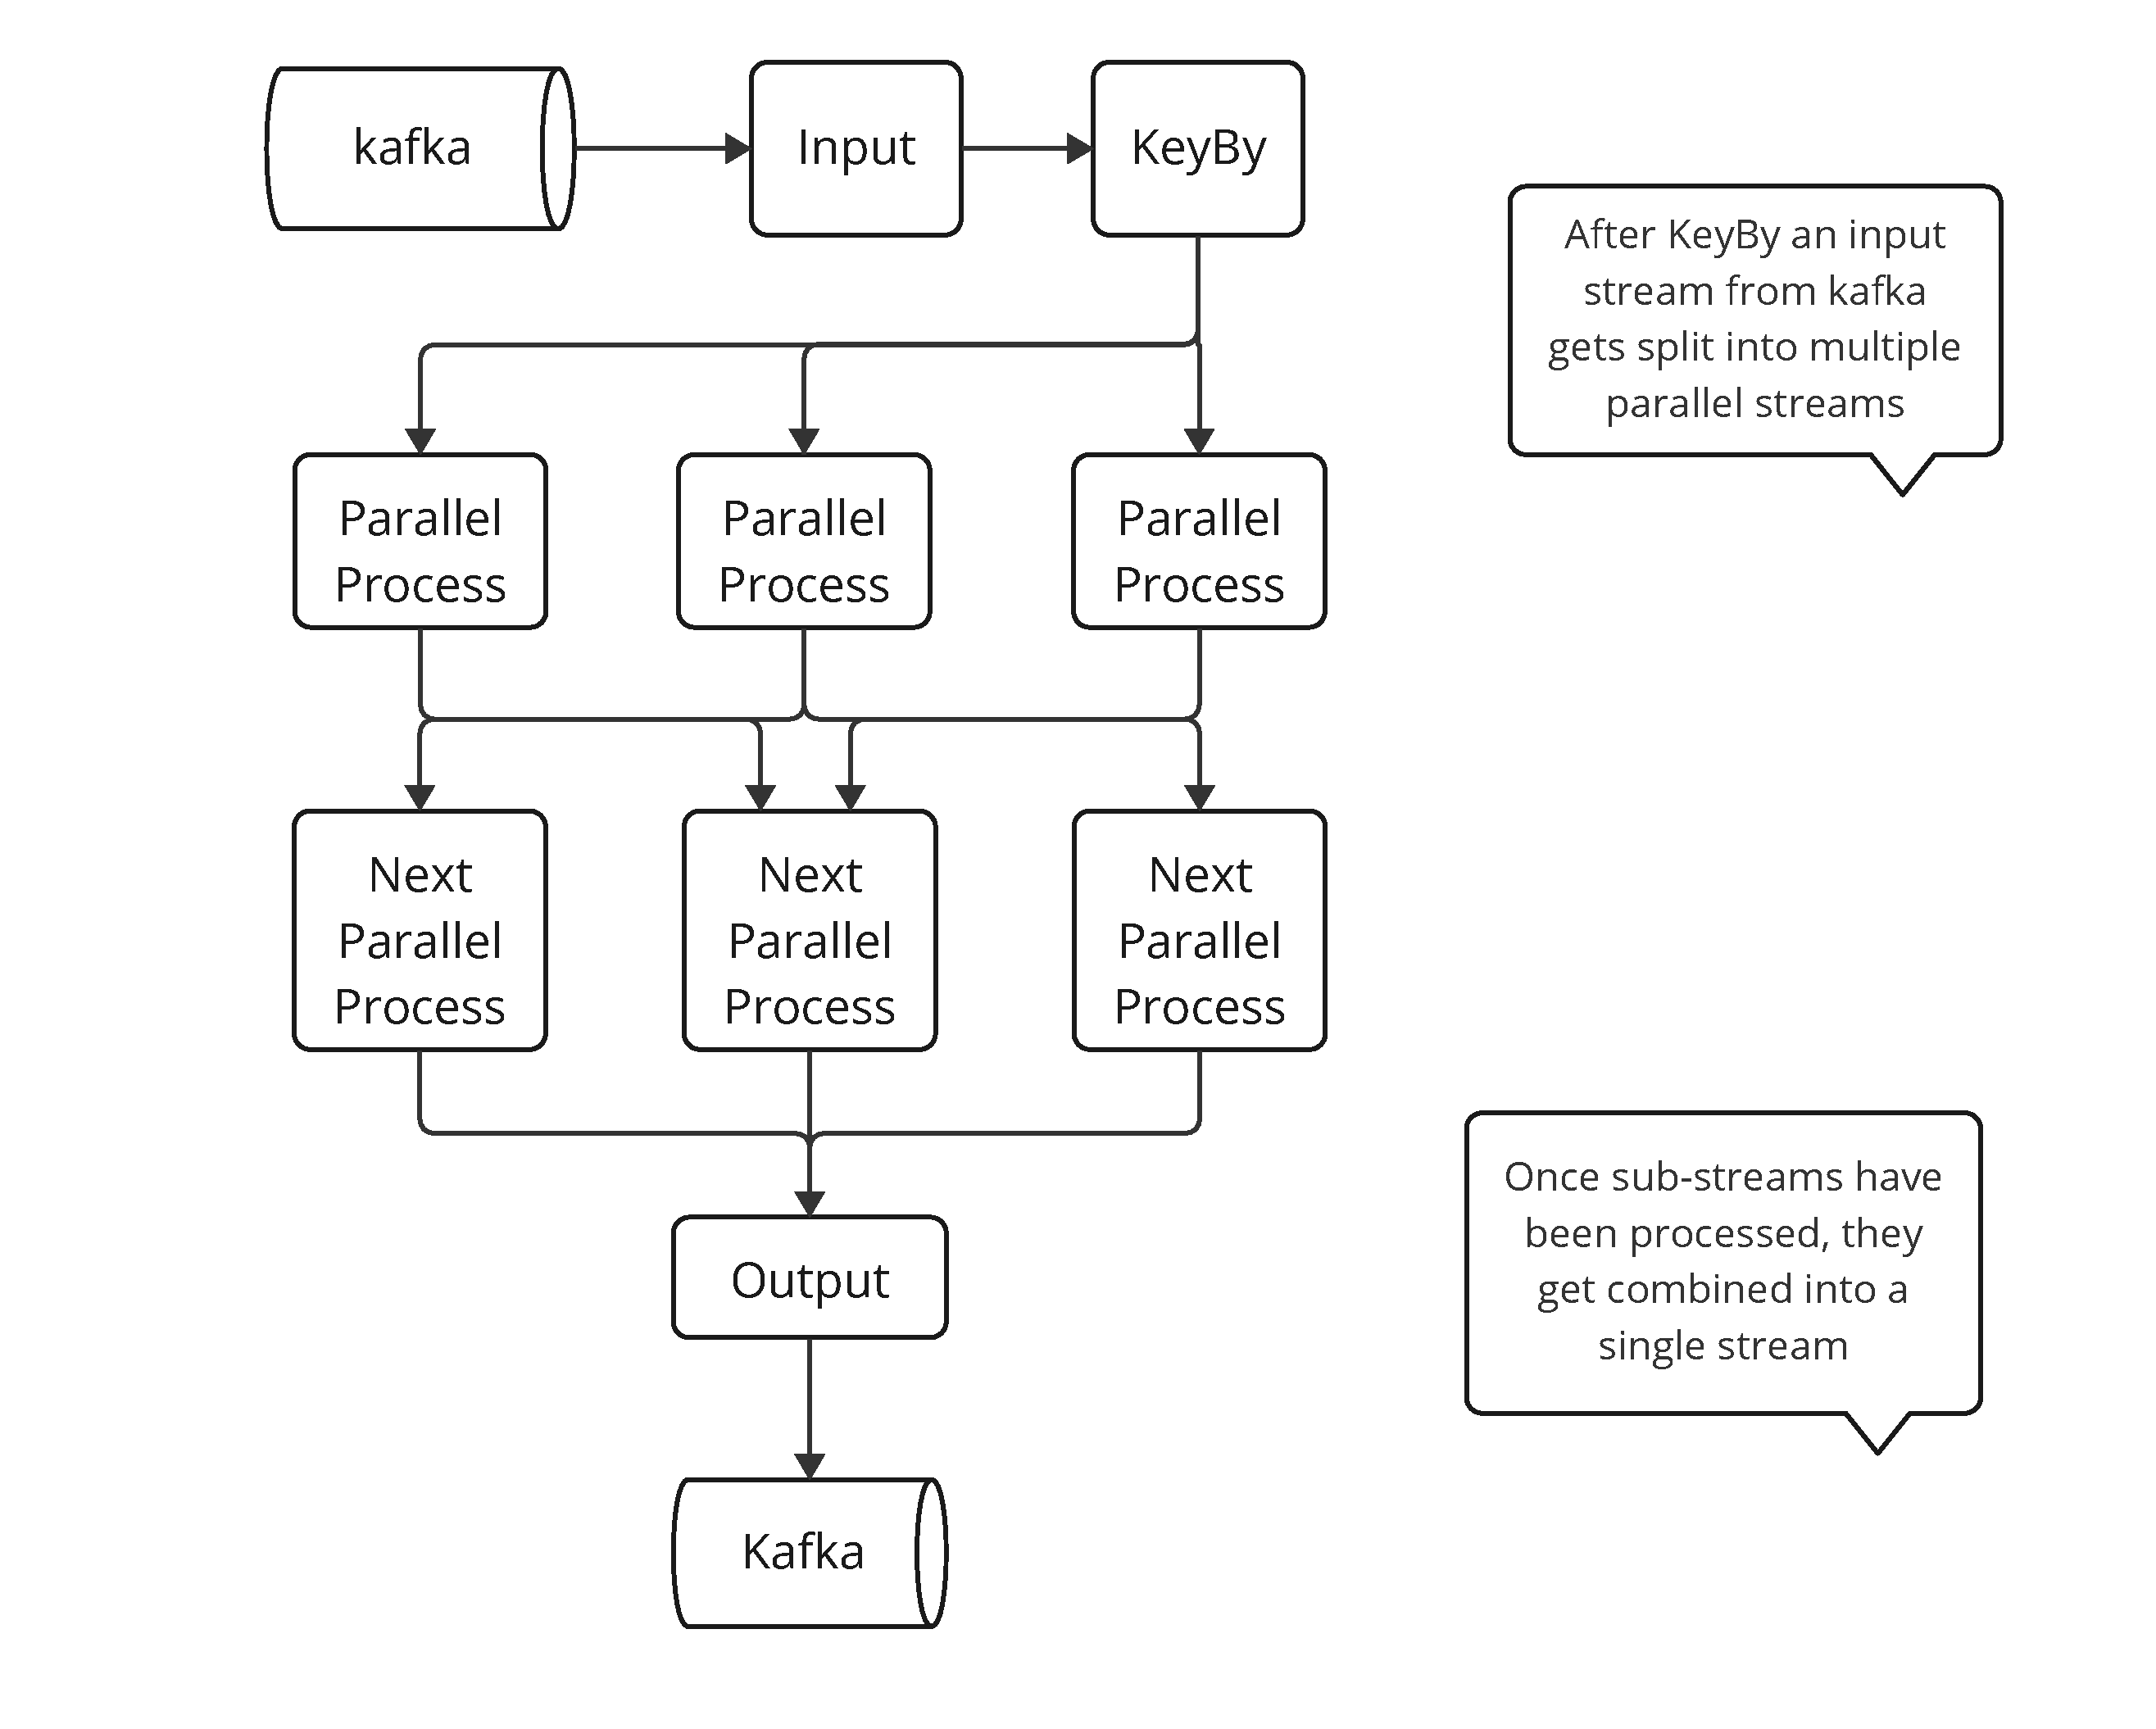
\includegraphics[width=1\textwidth]{figures/dataflow-graph}
    \caption{\textit{An example of data stream execution with dataflow graphs.}}
    \label{fig:dataflow-graph}
\end{figure}

\newpage

\subsection{Data Parallelism and Task Parallelism}\label{subsec:data-parallelism-and-task-parallelism}
Data parallelism and task parallelism might sound confusing even for experienced developers.
In dataflow graphs, parallelism can be achieved in two ways.
Data parallelism with partitioning input data and executing tasks of
the same operation on data subsets in parallel, allowing for efficient processing
of large data volumes and spreading the computation load across multiple computing nodes.
Task parallelism, on the other hand, refers to tasks from different operators
performing computations on the same or different data in parallel,
which enables better utilization of the computing resources in a cluster.

\begin{figure}[H]
    \centering
    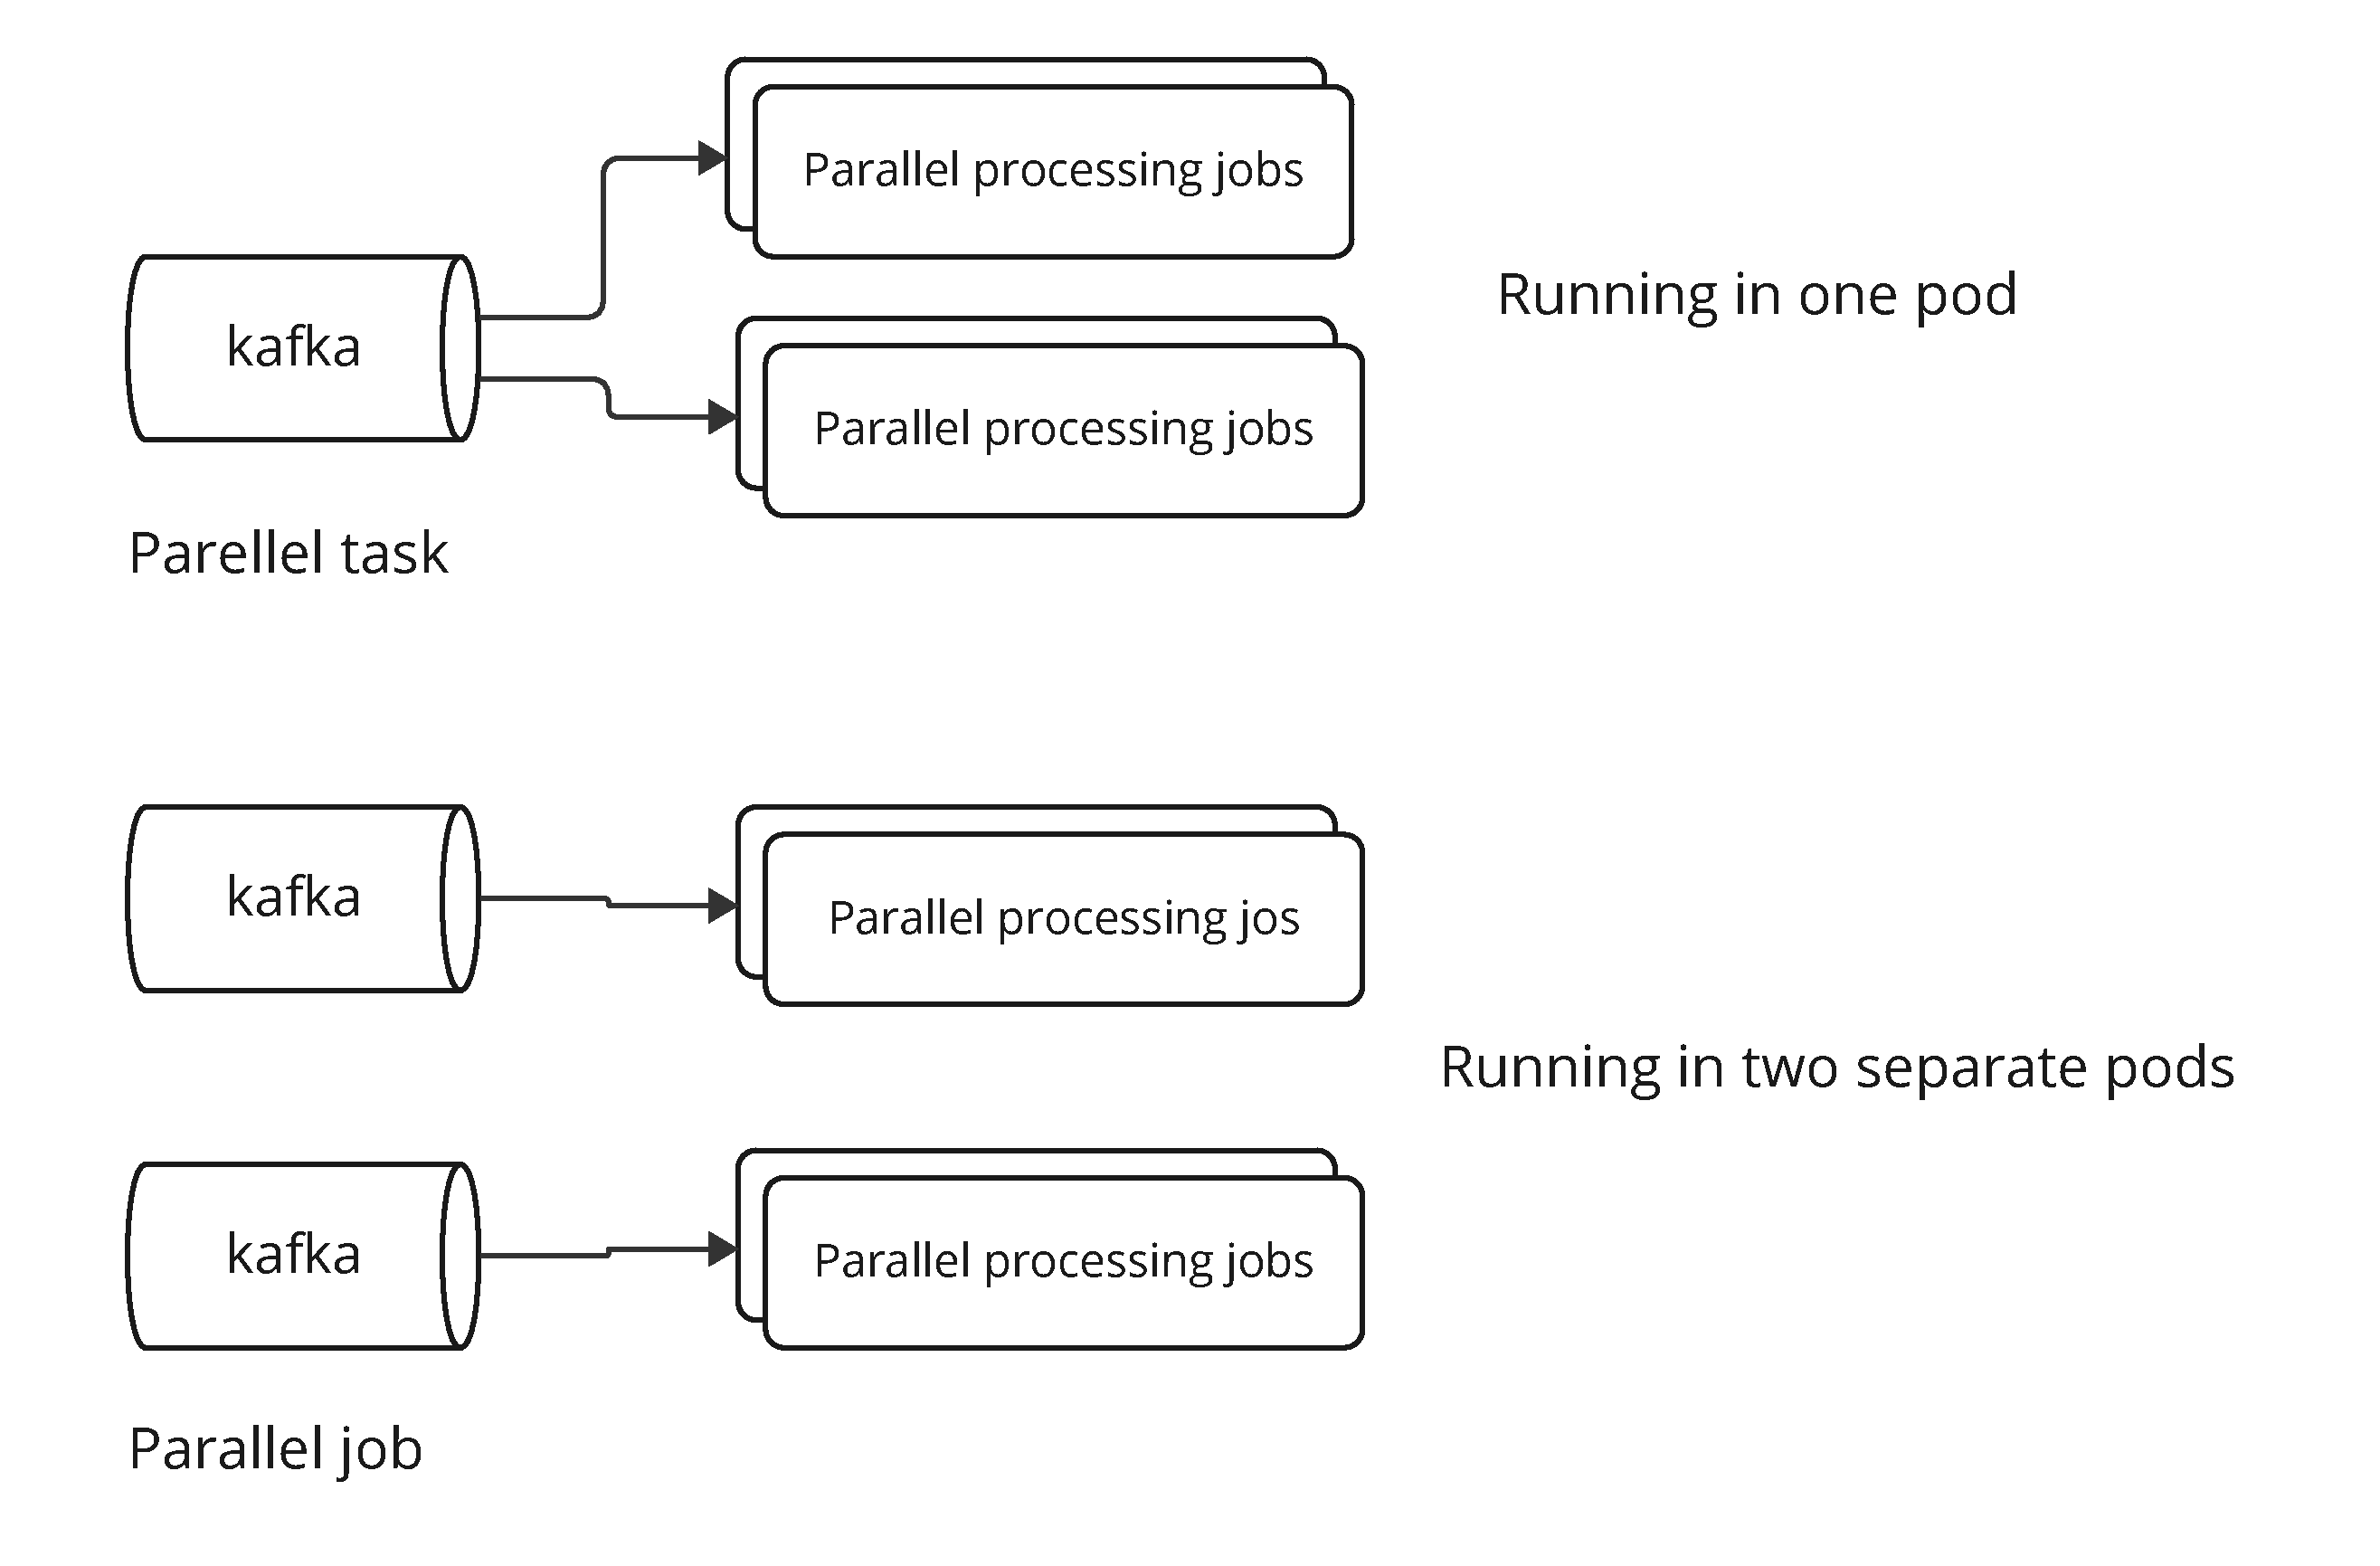
\includegraphics[width=1\textwidth]{figures/parallel-jobs}
    \caption{\textit{An example of data stream execution with dataflow graphs.}}
    \label{fig:parallel-job}
\end{figure}

In order to get better understanding, Figure \ref{fig:parallel-job} depicts a visual difference.
Job parallelism defined how many parallel task are running in separate execution node,
but performing as one single app.
In case of Kafka, each job's task processes a subset of kafka partitions, such
that all tasks process all partitions.
Kafka knows how to spread partitions among all tasks, a developer
don't need to worry about it, only if there's a very specific case for that.
In general partitioning should work automatically, the only a number of partitions
is under developer's responsibility.
There's a formula which defined a number of partition for a project which is getting started,
but as a data volumes grow it's good practice to add more partitions manually.
Moder monitoring tools help to identify such moment, when a number of partitions
should increase to handle new data volumes.

\subsection{Data Exchange Strategies}\label{subsec:data-exchange-strategies}

\begin{description}
    \item[Forwarding] The forwarding approach passes data straight from one task
    to the downstream task without reshuffling or rearrangement.
    The downstream operator processes data in the same sequence and partitioning
    as the upstream operator.
    Forwarding is the most efficient strategy, due to less overhead and network communication.
    \item[Partitioning] Data is redistributed among parallel jobs depending on a key or function.
    Key-based partitioning, which shuffles and groups data by key values, is the most frequent.
    Keyed aggregations, joins, and groupBy use this method.
    Partitioning processes all records with the same key.
    \item[Broadcast] Data from upstream jobs is replicated and delivered to downstream activities.
    In a broadcast join or when a small dataset needs to be available to all downstream
    for processing, then broadcast strategy is used.
    \item[All-to-All] The all-to-all technique sends all upstream records to all downstream jobs.
    This method is utilized when data order or partitioning doesn't matter
    or when every task must process the complete dataset.
    For large datasets, this method has a substantial transmission overhead.
    \item[Rebalancing] Rebalancing redistributes data evenly across downstream processes.
    It prevents data skew and load imbalance from uneven data distribution.
    Rebalancing guarantees that downstream tasks receive roughly the same quantity of records,
    improving performance and resource use.
    \item[Random] Random uniform distribution across downstream tasks.
\end{description}


\begin{figure}[H]
    \centering
    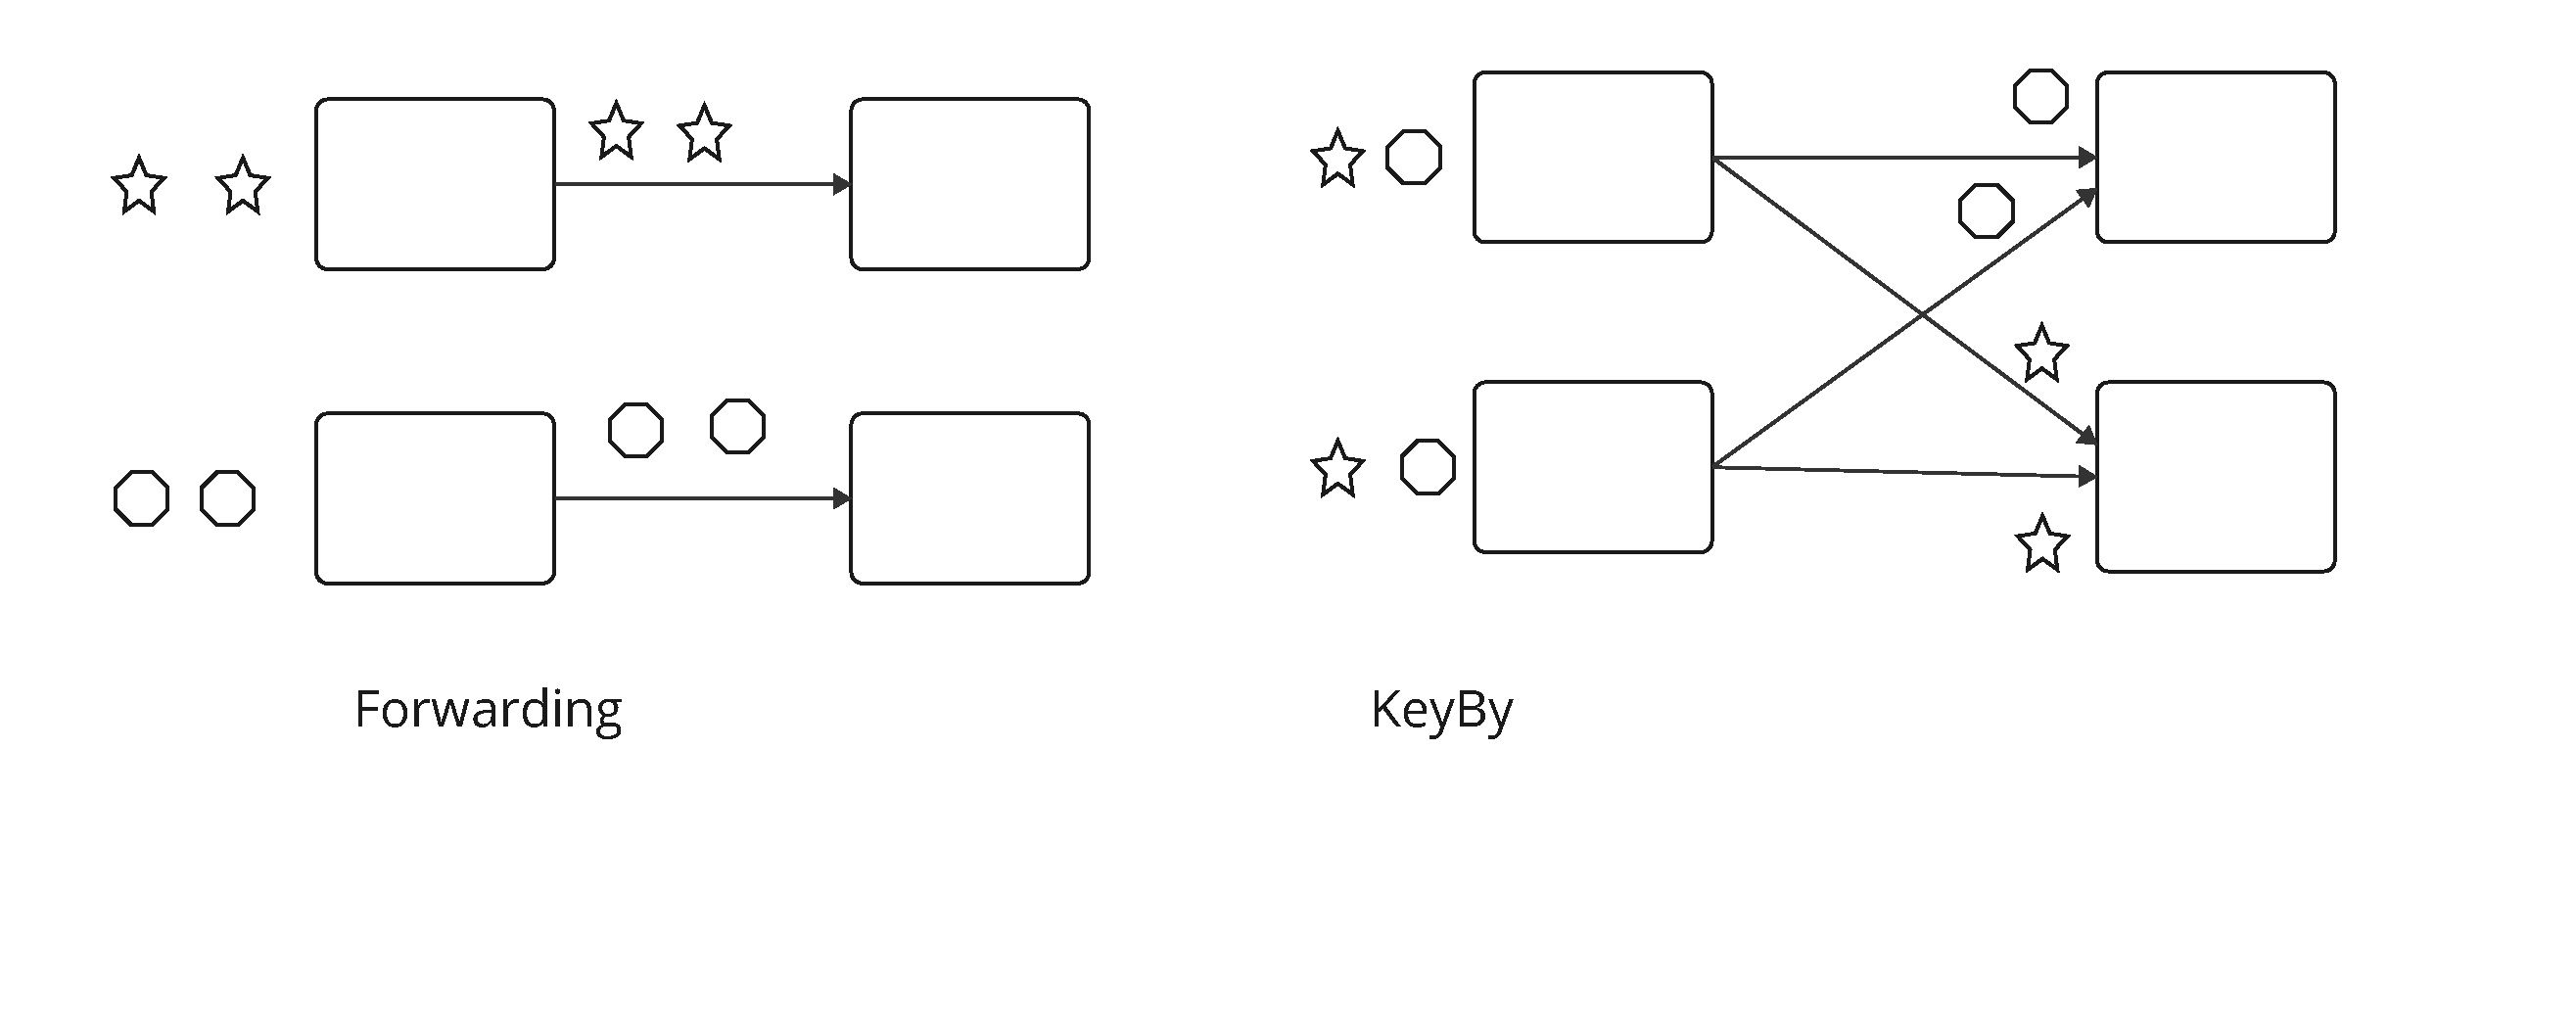
\includegraphics[width=1\textwidth]{figures/forward}
    \caption{\textit{An example of forwarding and partitioning by key.}}
    \label{fig:forward}
\end{figure}

\newpage
\section{Stream processing: challenges}\label{sec:-challanges}
Since this research is focusing on stateful streaming,
a variety of challenges must be handled by a new solution.

\begin{description}
    \item[State Management] In the following context, a state represents a unit of information
    which can saved, accessed and updated by a key.
    For example a key based counter.
    In a distributed streams,
    updating and accessing state might be difficult.
    Operators must ensure consistency and minimal latency while managing
    state across multiple jobs and nodes.
    In order to handle state efficiently, sharding, partitioning,
    and replication must be used.
    \item[Fault tolerance] fault tolerance was already covered earlier as a requirement.
    It's also quite challenging since different frameworks have different strategies for 
    recovery.
    \item[Scalability] Scalability also was covered earlier as a requirement, scalability
    as a fault tolerance are done differently for streaming frameworks.
    \item[Rebalancing] Balancing is a core feature which deals with fault tolerance
    and scalability the same time.
    There are difference options, which are configurable.
    Kafka provides a great api for a flexible setup.
    In this case it's important to sync with business requirements.
    Balancing will be covered in details in the next chapter.
    \item [Processing latency] It is challenging, both Apache Flink and Kafka Stream are able
    to handle a load in a reasonable time range.
    \item[Exactly-once semantics] This challenge depends on a use case.
    Since exactly-once semantics is solvable with some tradeoffs  with a kafka, it
    will be covered in details in next chapters.
    \item[Deployment] At this time, streaming frameworks have already Kubernetes
    integration which allows to manage deployment and resources.
    Still some details might be challenging, like auto-scaling.
    At the beginning data processing frameworks were designed for deployment
    on YARN cluster.
    Step by step data frameworks have migrated to Kubernetes.
\end{description}

These challenges are most the important in this research, and in order to
understand how they can be solved I'll provide more details in the next sections.
Details for these challenges will be explained on top of the use case.

\newpage
\section{Kafka as a stream data provider}\label{sec:kafka-as-a-data-provider:-challenges}
The use case which will be evaluated in this research is supposed to work with kafka which
provides a source of unbounded data stream.
Some developers might be confused about terminology and a difference
between kafka and kafka streams.
This section is trying to describe Kafka components and describe what is important
for the thesis research.

\begin{description}
    \item[Kafka] is a distributed messaging system.
    \item[Kafka Streams] is a streaming library which is built on top of Kafka.
\end{description}

From a very generic view Kafka represents a message queue and consists
of 3 core high level components which are Consumer, Producer and Broker.

\subsection{Producer}\label{subsec:producer}
Producer is an application that sends data
records to Kafka topic.
Kafka records can obtain any form of data, including log files, user activity, and sensor readings.
Producers must decide which partition within a topic to send messages to,
either through a round-robin approach or by establishing a partitioning strategy
depending on the message content, for example by record key or by custom balancing strategy.
Kafka provides producer api client which is used withing an application.

\begin{figure}[H]
    \centering
    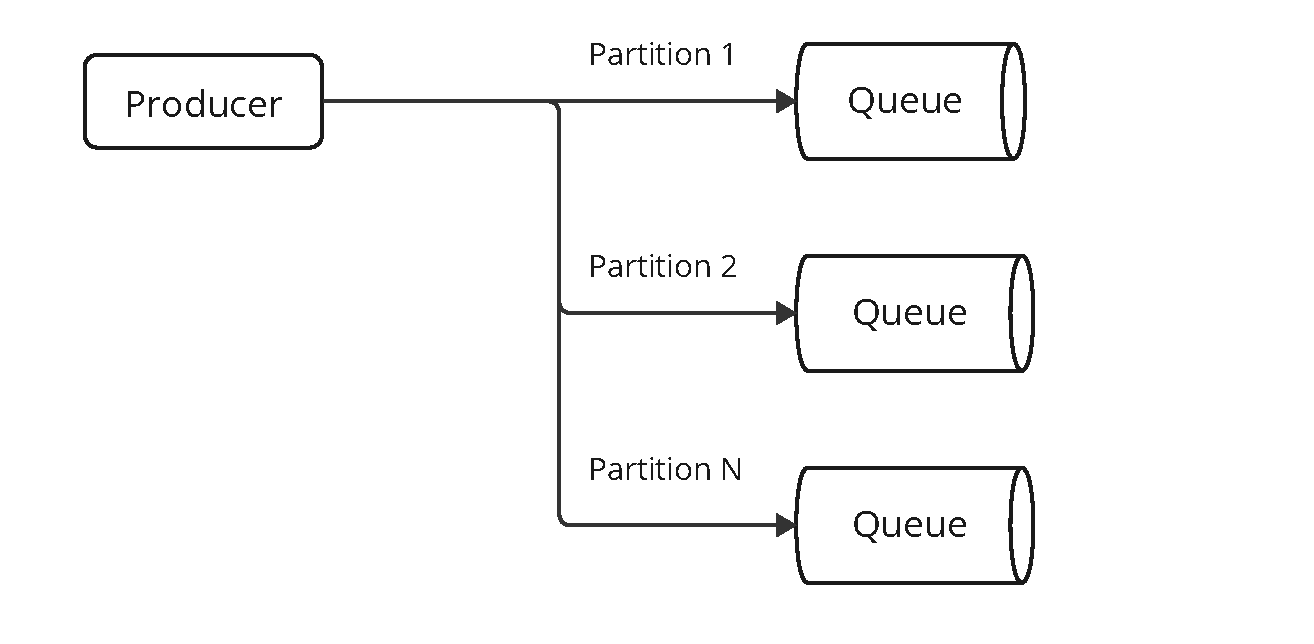
\includegraphics[width=1\textwidth]{figures/producer}
    \caption{\textit{An example of forwarding and partitioning by key.}}
    \label{fig:producer}
\end{figure}

Figure \ref{fig:producer} shows a common producer model which sends
records to Kafka topic which has two partitions.
In case of multiple partitions, Kafka provides multiple
balancing strategist.
A strategy selection depends on a business requirements and a use case.
Down below are described three possible scenarios for balancing.

\begin{description}
    \item[Record key is not specified] In this case producer use Round robin strategy
    and sends records for using each partition subsequently,
    For example, is there are two partitions, first message goes to partition 1,
    seconds to partition 2, third goes to partition 1 and etc.
    \item[Specified partition] A developer explicitly defines a partition to send.
    \item[Partitioning with hash function] Hash function uses a record key as
    an in input parameter hash output specifies a partition.
    Hash function must deterministic, it means that one key has always the same partition.
\end{description}

For the research use case it was decided to go with the Round robin balancing
since a record is supposed to be 1Kb byre array which has no key.
This allows kafka producer to balance records quite efficiently.

\newpage
\subsection{Consumer}\label{subsec:consumer}
[Consumer] is application that consumes messages from Kafka topic.
As with producer, kafka api also provides consumer api client.
Consumers are members of consumer groups, which enable them to share
the processing load and read messages concurrently.
keep track of their progress by saving the offset of the most recent
message they have consumed.
Each message in a partition is given a distinct offset.
In case of balancing, offset has a pointer which indicates which latest record was consumed by
a consumer.
If several consumers consume the same topic then kafka broker creates two offsets for
each consumer


\begin{figure}[H]
    \centering
    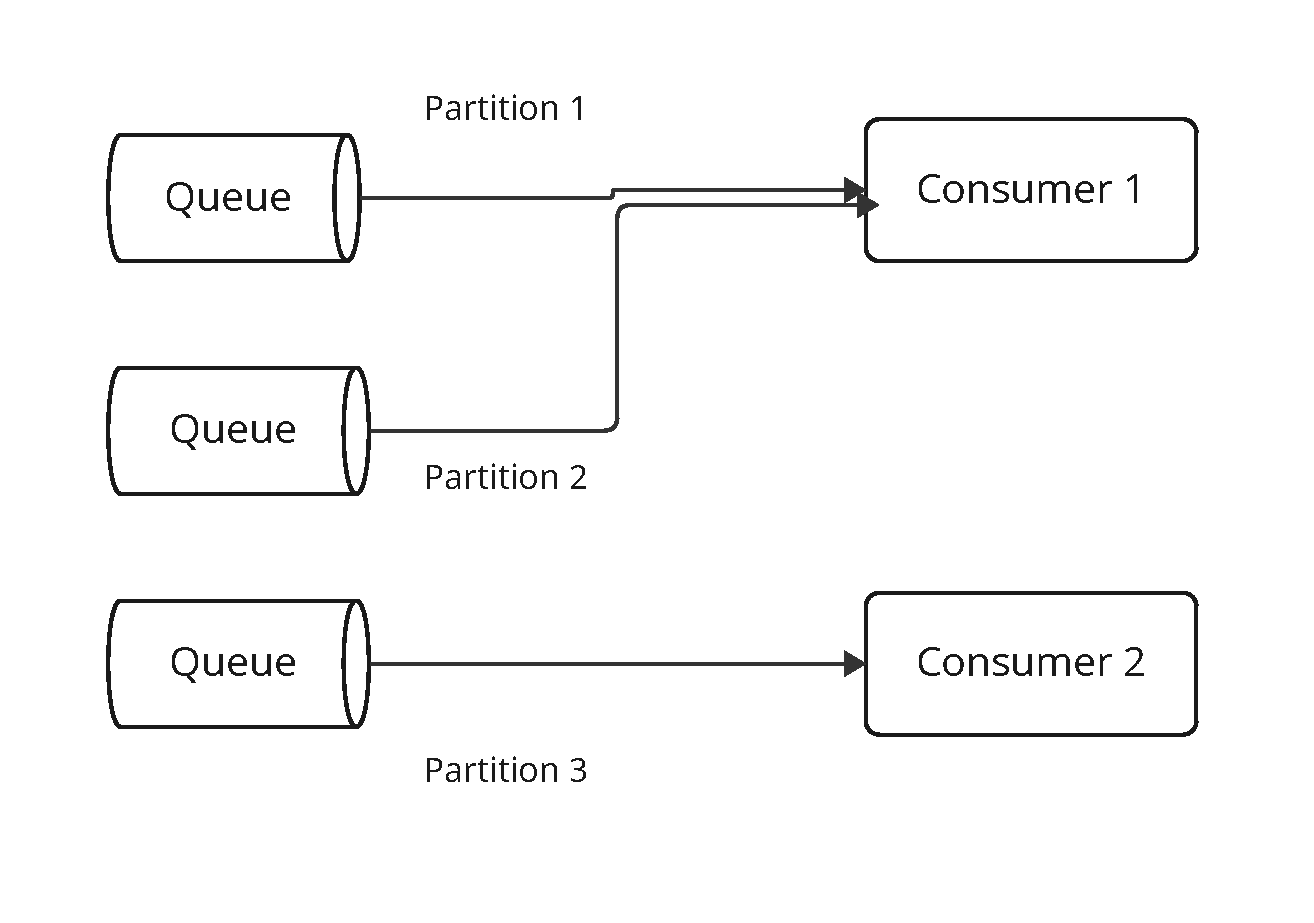
\includegraphics[width=1\textwidth]{figures/consumer-kf}
    \caption{\textit{An example of forwarding and partitioning by key.}}
    \label{fig:consumer-kf}
\end{figure}

Figure \ref{fig:consumer-kf} show a case for three topic partitions and two consumers.
It can be seen that in this case the first consumer consumes two partitions.
In case of one partition, the only one consumer would receive a data stream,
the second would work in idle mode awaiting new available partitions.
Partition assignment is fully managed by the Kafka broker which is described
in the next section.

\newpage
\subsection{Kafka Broker}\label{subsec:kafka-broker}
Kafka broker is a central component of Kafka ecosystem.

Its main responsibilities are:

\begin{description}
    \item[Processing record queus] Each broker manages one or more partitions for each topic.
    When producer sends a record to Kafka topic, the broker stores records
    in the corresponding partitions, which represents multiple queues.
    Each record is assigned to incremental offset within its partition,
    which helps in maintaining the order in which record were written.
    Kafka broker keeps record in a binary format which requires developers
    to implement a corresponding serializer for producer and deserializer for consumer
    if a standard set of serializers and deserializers do not work.
    \item[Replication] To ensure fault tolerance and high availability,
    brokers replicate the data across multiple replicas.
    These replicas are distributed across different brokers in the cluster.
    In case a broker goes down, another broker with a replica of the same data can take over,
    ensuring that no data is lost.
    Replication factor is set by a Kafka cluster administrator.
    \item[Consumer managetment] Broker enable consumers to read records from the Kafka topics.
    The broker makes sure that
    consumers can subscribe to one or more topics and read records
    in parallel by being part of a consumer group, it
    helps consumers track their progress by maintaining
    the offset of the last consumed record.
    More cases will be described in the section which is dedicated to
    processing failures.
    \item[Load balancing] Multiple brokers work together to distribute and balance the processing load.
    As the number of topics, partitions, and replicas increases,
    the Kafka cluster can scale horizontally by adding more brokers.
    This ensures that the system can handle increasing data throughput and storage requirements.
    It's important to know that Kafka administrator has to have a full monitoring
    to be able to properly scale the system by having access to Kafka Admin api.
\end{description}

Kafka clustering is a crucial work of this research, since a quite complex infrastructure
is involved into benchmarking experiment.
Moreover, a group of brokers is involved, to simulate setup Kafka cluster the way
it's running in a production.

\newpage
\subsection{Kafka alternatives}\label{subsec:kafka-alternatives}
Obviously, Kafka is not only the one message broker, there are alternatives.
First at all, cloud service providers such as AWS, Azure, Google Cloud
provide their own solutions like Azure Event Hub, Big Query, Amazon Kinesis.
It's indeed, quite convenient to use already made for use solutions, but
the main requirement is to be independent of cloud streaming solutions.
Cloud based streaming solutions is not only the one alternative but there
are more open source solutions.

\begin{description}
    \item[Redpanda] Looks like quite promising solution indeed.
    But has a several drawbacks which are crucial at the moment, maybe in
    a couple of years everything will change.
    Among drawbacks when comparing Redpanda as alternative data stream solution
    is its C++ infrastructure.
    Which would require additional engineering requirement for the who's
    responsible for the infrastructure, since it based on different programming
    language which also means additional complexities for production deployment.
    Another important fact is that Kafka has a really large open source community
    and a solid documentation.
    Redpanda might a good solution for a latency critical use case or integration with
    embedded systems.
    \item[Apache Puslar] Which also works as a data streaming solution.
    It's not quite clear how effect exactly-once semantics would work,
    requires additional PoC solution with tests.
    Additional integration with Apache Flink, and there's no such functionality
    as Kafka Streams provides.
    It only means that for research use case it is not a great fit, but for other use cases
    would work better.
\end{description}

As a summary, for research use Kafka is great fit due to existing JMV
infrastructure, needed features are presented and huge community support.


\newpage
\section{Comparing Kafka Streams and Apache Flink}\label{sec:kafka-vs-flink}
In this section Kafka Streams and Apache Flink are compared for their
feature set which are important for the use case.
It might be to that trivial task consider how well they behave and are considered as
industry standards for stateful streaming.


\subsection{Input and Output}\label{subsec:input-and-output}
When considering frameworks, one of the first requirement comes
with integration possibilities.
Fortunately, modern data processing frameworks come with a set of
input output integration modules.
This set if different depending on framework.

\begin{description}
    \item[Kafka Streams] fully relies on Kafka.
    Kafka Streams always uses kafka topic as input and kafka topic as output.
    It means that any kind of integration, either database, or csv data, it must
    be transformed to kafka topic.
    Kafka provides a set of kafka connect modules which provide an integration with
    different sources, but it takes additional kafka resources and kafka connect setup.
    For research use case, the data is coming from a kafka topic which makes it ease to use.
    \item[Apache Flink] supports different kinds of data sources byt built it functionality,
    moreover Flink functionality provide a transactional data source integration.
    Flink provides wider options for native data source integration which makes it
    a good choise if custom data source is required.
\end{description}

Since research use case uses Kafka as a data source both
Kafka Streams and Apache Flink would fit well.


\subsection{Parallelism}\label{subsec:topology}
Both Kafka Streams and Apache Flink use a dataflow graphs, but they
have a different parallelism setup.

\begin{description}
    \item[Kafka Streams] uses dataflow graph topology which provides a great scalability.
    To make stream processing scalable, it's required to have more parallel application
    processing units.
    Where each pod is responsible for a set of partitions defined by Kafka brokers.
    \item[Apache Flink] uses dataflow graph topology but provides different
    parallelism model, which is mode advanced comparing to Kafka Streams.
    Flink provide processing slots with the task manager, such that, Flink
    allows to set up parallelism within a processing unit and parallel processing units.
\end{description}

As a summary two processing Apache Flink units with 2 slots provide parallelism with factor 4,
however Kafka Streams would require 4 processing units.

\subsection{State management}\label{subsec:state-management}
One of the requirement for the streaming processing solution is exactly-once semantics.
Both frameworks allow to implement a stream processing with exactly-once semantics,
but it might by challenging for failure recover cases since Kafka Streams and
Apache Flink keep state in its recovery differently.

\begin{description}
    \item[Kafka Streams] uses kafka topics to keep and manage states.
    It provides a great advantage for recovery cases since topics
    are distributed, another Kafka Streams instance can take responsibility
    of a state which was being processing in failed processing unit.
    \item[Apache Flink]
\end{description}

\chapter{Methodology}\label{ch:second_chapter}
This chapter describes experiment setup and performance evolution methods that are
used to demonstrate performance difference.


\section{Introduction}\label{sec:introduction}


%\subsection{Overview}\label{sec:overview}
This chapter describes the methods that are used in this research.
The main goal of the thesis is to figure out how Apache Flink and
Kafka Streams behave and perform, what configurations are needed,
and how to solve fault tolerance problems in case of a stateful streaming.
They both are designed for use in a streaming domain, but there must
be some difference in how they perform and get configured to run in the Kubernetes cluster.
The key moments for both systems are scalability, resilience, fault tolerance,
cost efficiency, setup complexity, documentation, and learning curve.
To get experiments running, it is crucial to get an execution environment,
especially for big data solutions, which are not possible to run on a laptop.
Big data solutions and benchmarks require a cluster of hardware machines that represent nodes.
For this reason, all the benchmarks and execution environments are done with AWS and EKS in particular.
AWS provides services such as Amazon Managed Streaming.
It solves a lot of configuration problems, but it adds additional cost.
It should be suitable for less-loaded streaming solutions where load demand is not that
big and there’s no dedicated team.
Heavy-loaded services where latency is also essential rely on their own Kafka cluster setups
and streaming setup, such as Spark Streaming or Apache Flink.
These experiments are based on the execution configuration provided by the Theodolite framework.
Theodolite provides an essential customizable Kafka cluster setup,
which is easy to reconfigure and has more control over running experiments,
making it easy to deploy infrastructure in EKS \cite{AWSEKS2024}.
Theodolite \cite{theodolite_framework}, a robust framework, plays a pivotal role in acquiring measurable benchmarks.
It offers a suite of tools, including Grafana \cite{Grafana2024} and Prometheus Operator \cite{PrometheusOperator2024}.
These tools are equipped with ready-to-use and configurable Prometheus \cite{Prometheus2024} pod monitoring agents,
enabling the collection of various metrics from running pods within the EC2 node \cite{aws_node_types} \cite{EC2}.
The Theodolite operator, in conjunction with Prometheus and Grafana,
is specifically designed for easy deployment in a Kubernetes cluster environment,
providing super low latency real-time metrics.

One of the most important step is a data analysis, which is also possible using Theodolite framework
since it provides metrics export interface.
All the recorded metrics will be analysed using Python libraries and tools
\cite{hightower2019kubernetes} \cite{pivotto2023prometheus} \cite{theodolite_framework}.


\section{Research Technical Tasks}\label{sec:research-objectives}
Two frameworks, Apache Flink and Kafka Streams, are written in Java and designed to run in a cloud environment.
Both prototypes are written in Java.
For experiments,  AWS was chosen since it is one of the most advanced cloud providers.
AWS provides services for running scalable streaming solutions such as EBS \cite{awsEBS}, EFS \cite{awsEFS}, EC2 \cite{EC2}, EKS \cite{AWSEKS2024}.
The research is split into following steps:

\begin{description}
    \item[Prototypes development] Development of two Java based prototypes with Apache Flink and
    Kafka Streams which process the same input and send result to the same output.
    Both prototypes are based on Java 11.
    Input and output are Kafka topics with 50 partitions.
    \item[Tools selection] AWS as cloud provider, EKS as kubernetes cluster, Theodolite \cite{theodolite_framework}
    \cite{applications_benhcmarks} that is one of the most advanced frameworks for setting up streaming benchmarks
    in cloud environment.
    Theodolite includes out of the box Grafana \cite{Grafana2024}, Prometheus \cite{Prometheus2024} \cite{PrometheusOperator2024}, Kafka \cite{kafka_intro}, Apache Flink and Kafka Streams cloud
    benchmarking cloud configurations provides as Helm charts \cite{helm}.
    Chaos Mesh \cite{chaosMesh} is chosen as it provides scheduled job failures in a cloud environment.
    \item [Kubernetes cluster design] The cluster must have different node groups for different components.
    For this study were used 3 main node groups, worker node group, infra node groups, generator node groups, depicted on Figure \ref{fig:node-gorups}.
    \item[Metrics definition] Metrics include node network traffic, CPU consumptions, consumer group lag,
    lag for each partition, state recovery time.
    All metrics are implemented with PromQL \cite{prometheusQuerying}.
    \item [Experiments execution] All experiments are defined with Theodolite execution files \cite{theodoliteExecution}
    that allows to rerun experiments with the same execution conditions.
    \item[Results collection] Results from PromQL execution are saved in Kubernetes by Theodolite as scv files.
    \item[Results analysis] CSV files get analysed with Matplotlib Python library.
\end{description}

\begin{figure}[ht]
    \centering
    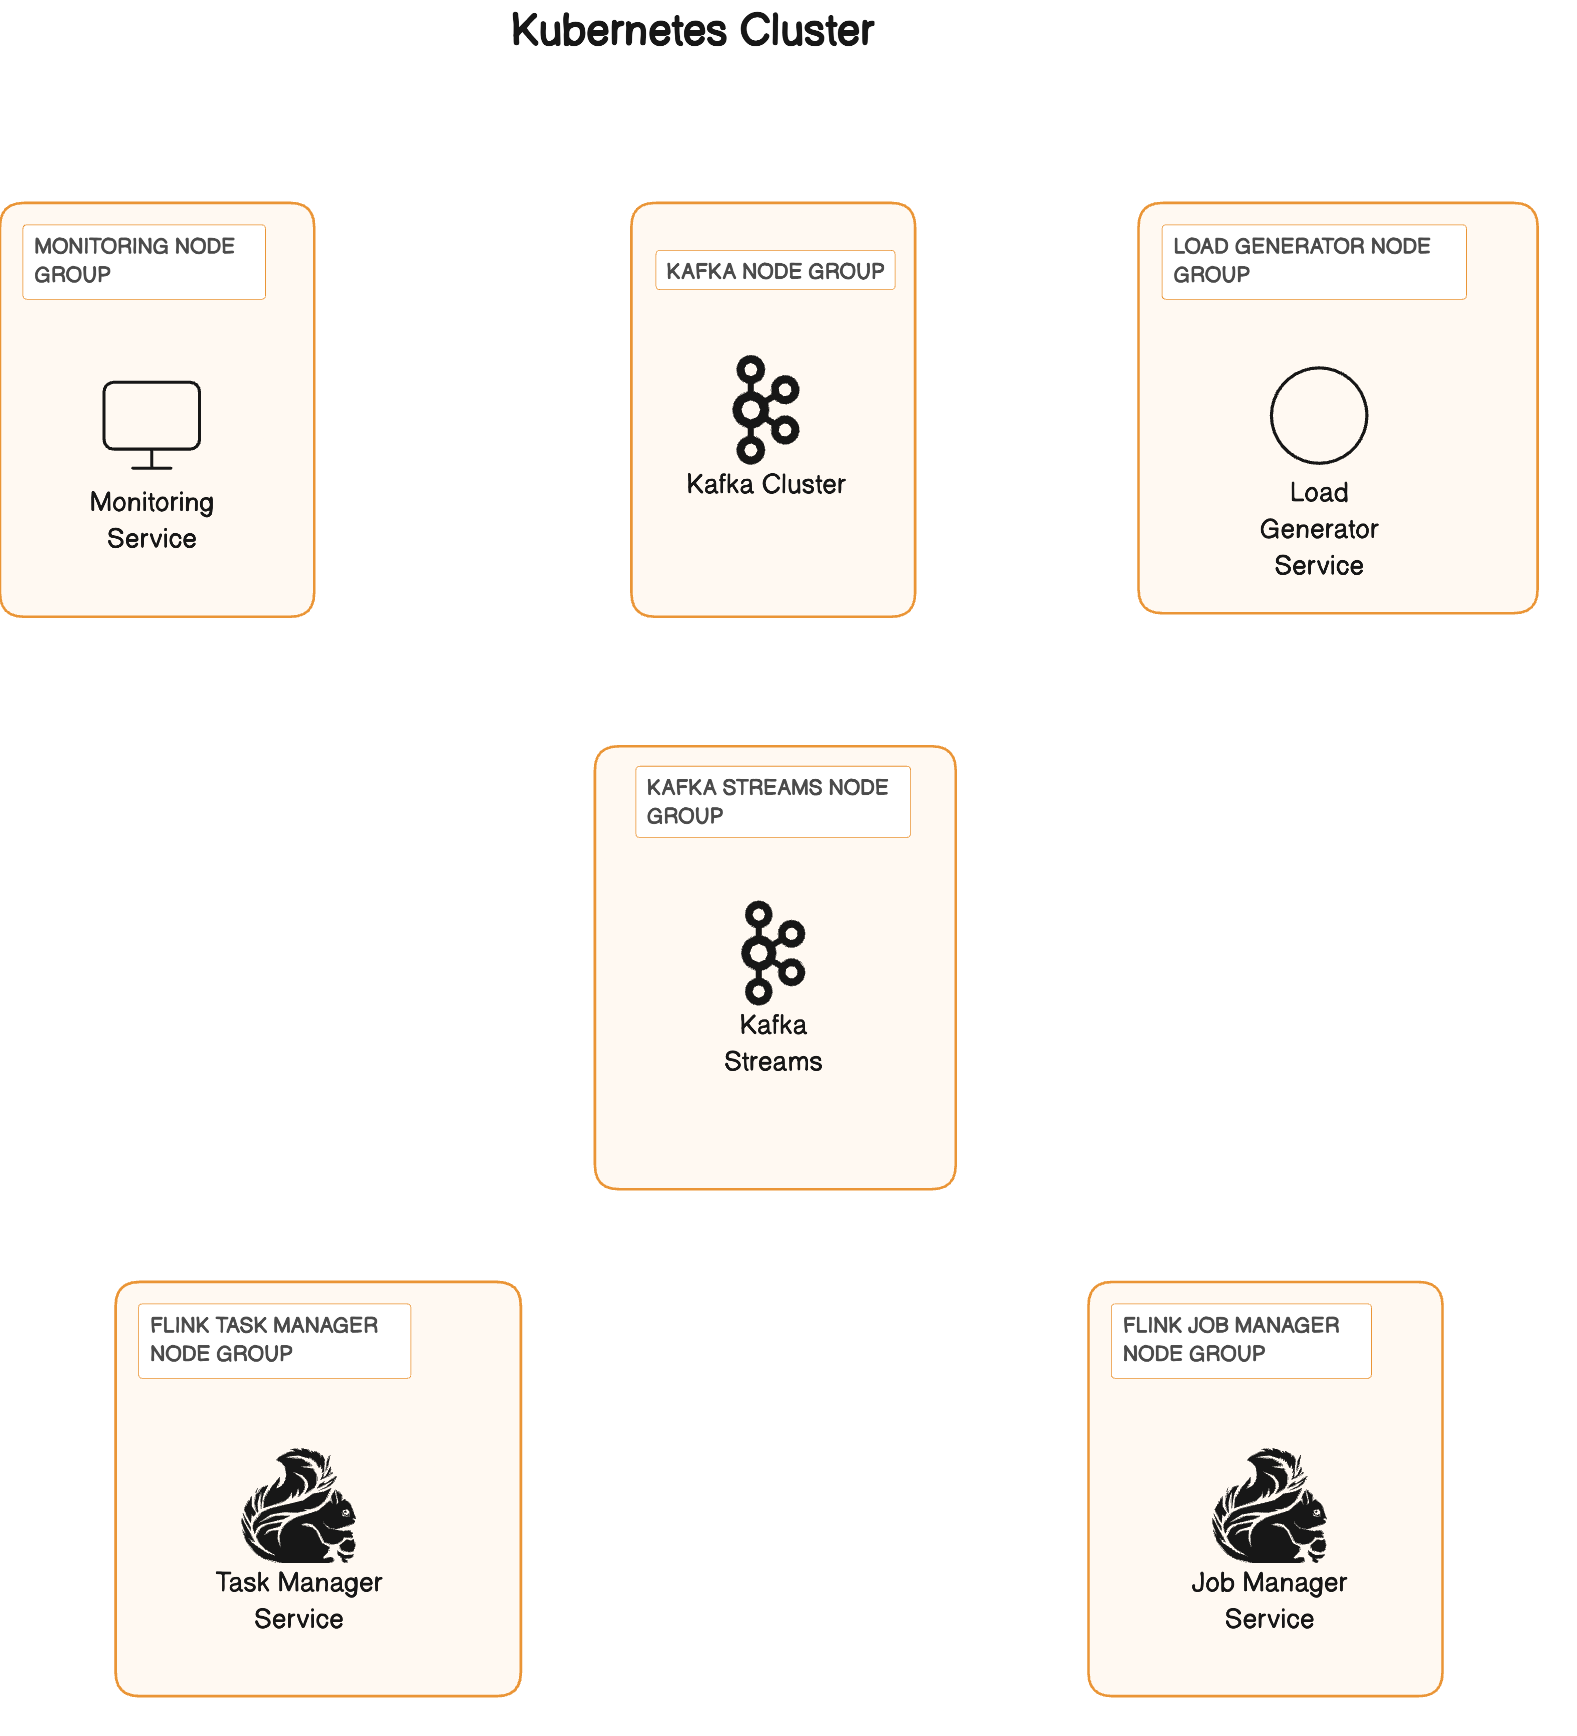
\includegraphics[width=1\textwidth]{figures/eks-node-groups}
    \caption{\textit{Node groups for the case study experiments.}}
    \label{fig:node-gorups}
\end{figure}


\newpage
\section{Kubernetes Cluster Setup}\label{subsec:eks-cluster-configuration}
This section is describing Kubernetes cluster and key components which are running
with during experiments execution to collect metrics.

\subsection{EKS Node Groups}\label{node-groups}

As shown on Figure \ref{fig:node-gorups}, the setup is based on 5 node groups and EC2 nodes \cite{aws_node_types}.

\begin{description}
    \item[Kafka node gorup] 3 Kafka brokers, where each broker gets deployed to a separate node.
    Such that several brokers never run on the same node.
    Node types for this group is m6i.2xlarge \cite{aws_node_types}.
    \item[Load generator node group] Is Java based application which generates Kafka messages of 1Kb size
    to Kafka input topic with 50 partitions.
    In this study two load generator instances are used where each generates 100000 messages per second.
    Node types for this group is m6i.xlarge.
    \item[Manager node group] The following node groups is intended only for Apache Flink task manager \cite{flinkArchitecture2024} instance of 1 replica
    and is not used for experiments with Kafka Streams.
    \item[Infra node group] This node group is used for benchmarking tools deployment such as EBS, EFS controllers,
    Grafana, Theodolite operator, Prometheus, Chaos Mesh and additional operators which are used only for data collection
    and visualisations.
    Should not affect workers and load generators.
    Node types for this group is m6i.xlarge.
    \item[Worker node group] This node group is used for Kafka Streams setup and Apache Flink task managers \cite{flinkArchitecture2024}.
    Such that stream processing replicas are running on a separate nodes, where each node has only one worker replica
    running in the node.
    Detailed worked groups is shown on Figure \ref{fig:worker-node-group}.
    For this case study were chosen 8 nodes with 8 workers replicas.
    Node types for this group is c5.large.
\end{description}


\begin{figure}[ht]
    \centering
    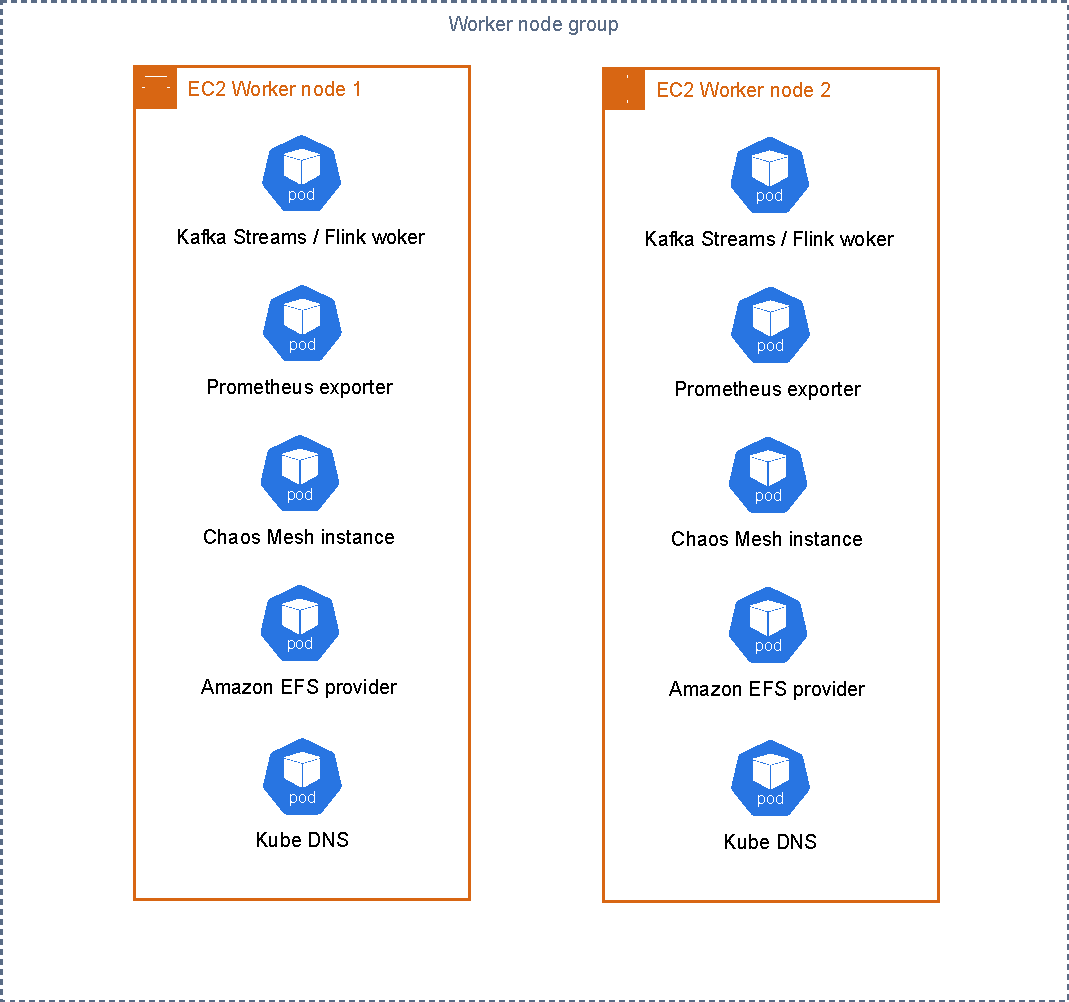
\includegraphics[width=1\textwidth]{figures/worker-node-group}
    \caption{\textit{Worker node group with 2 nodes and pods in each node.}}
    \label{fig:worker-node-group}
\end{figure}


\subsection{EFS and EBS Storage Services}\label{storage-services}

\begin{figure}[ht]
    \centering
    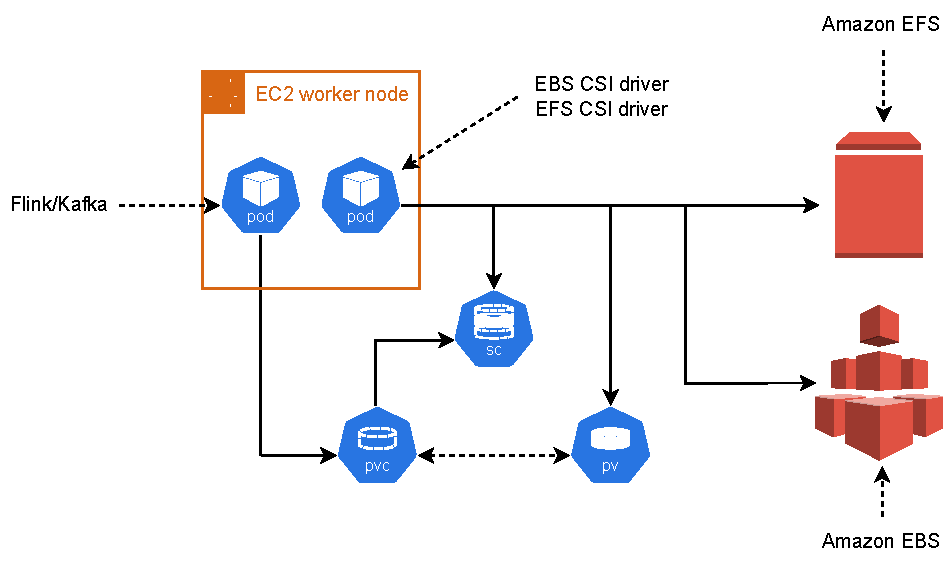
\includegraphics[width=1\textwidth]{figures/aws-storage-pvc}
    \caption{\textit{EBS and EFS network storage diagram.}}
    \label{fig:aws-storage}
\end{figure}

Stream processing uce case is data intensive in this study.
To be able to handle data loads during experiments were chosen two storage services
for storing the data.
These storage are EFS \cite{awsEFS}, and EBS \cite{awsEBS}.
AWS provides networks storage types for EC2 nodes \cite{EC2} which are used
for storing a big amount of data.
The crucial part of this network storage is that if worker on node goes down for some time,
then saved state won't be lost.
A real physical node is connected to the network storage via a network configuration as it shown on Figure \ref{fig:aws-storage}
which is also described in details in the following documentation \cite{awsKubernetesStorage}.
Such a complex model gives pod a network connection to a physical storage such that huge amount
of data gets written and read fast enough for production systems.
The diagram on Figure \ref{fig:aws-storage} includes several the following components.

\begin{description}
    \item[Flink and Kafka pods] These are Java application which use networks storage.
    For thi study Flink workers use EFS storage for storing stages and Kafka brokers
    use EBS for Kafka topics.
    \item[EBS and EFS CSI drivers] Cloud tool provided by AWS to manage network connection
    between nodes and networks storage.
    Driver runs on the same node as Kafka brokers and Flink worker to get network storage access.
    \item[PV] Persistent volume gives networks access to a physical storage, where the state gets saved.
    \item[PVC] Persistent volume claim is Kubernetes abstraction that connects to PV.
\end{description}


\section{Metrics Exporters}\label{sec:metrics-exporters}
This section cover how a Theodolite framework \cite{theodolite_framework} is used
to get metrics and to run experiments in cloud environment.

\subsection{Kafka Metrics Exporters}\label{subsec:metrics-exporters}
Theodolite comes with a set of tools which are used to export metrics from running pods.

\begin{figure}[ht]
    \centering
    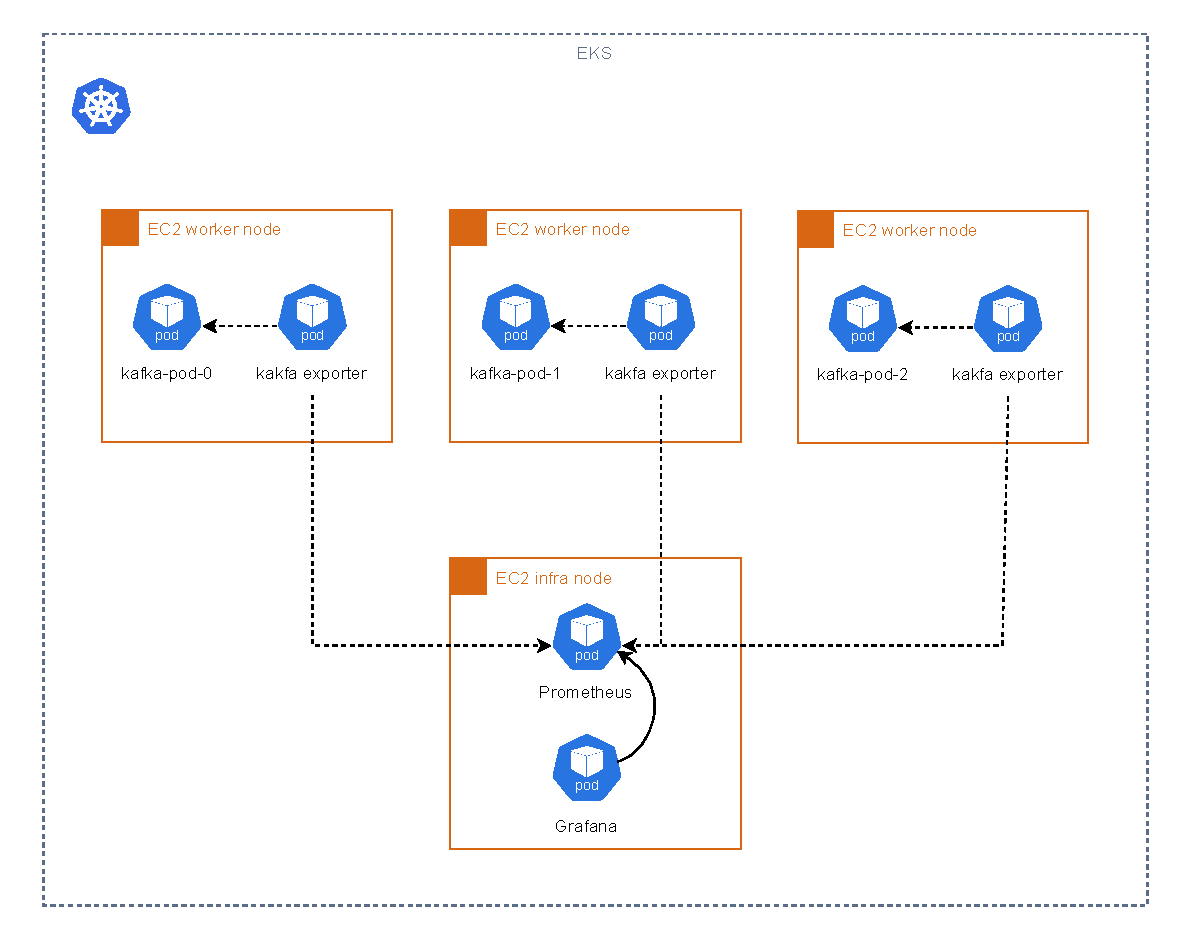
\includegraphics[width=1\textwidth]{figures/kafka-exporters}
    \caption{\textit{Kafka metrics exporter that sends metrics from JMX exporter to Prometheus.}}
    \label{fig:kafka-exporter}
\end{figure}

On Figure \ref{fig:kafka-exporter} is an example of Kafka metrics exporter.
It reads metrics from Kafka's JMX exporter about consumer groups, commit lag, topics,
topic partitions, topic offsets.

\newpage
\subsection{Kubernetes and Worker Metrics Exporters}
Kubernetes setup in this study is coming with Kubernetes metrics services \cite{kubernetesResourceMetrics} which are
configured by Theodolite.
Metrics diagram is depicted on Figure \ref{fig:metrics-collection}.

\begin{figure}[ht]
    \centering
    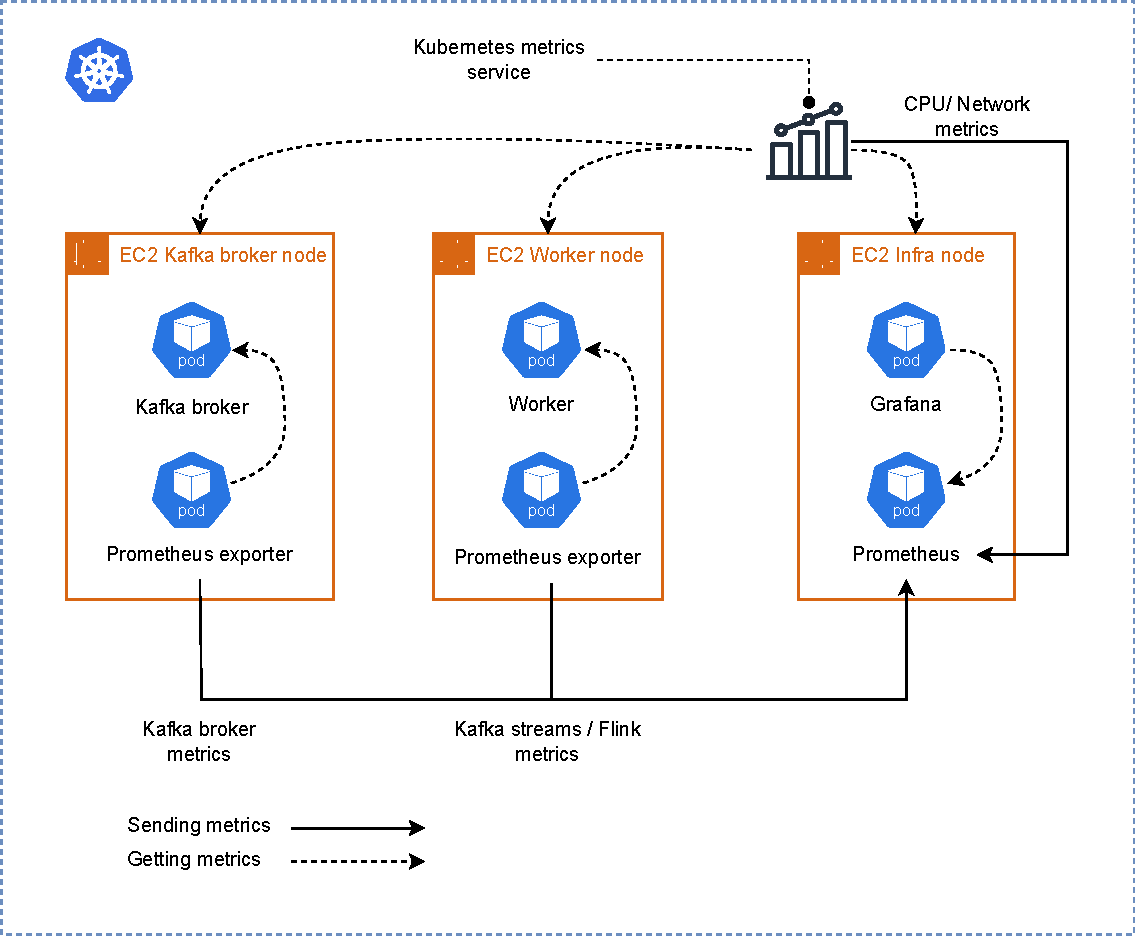
\includegraphics[width=1\textwidth]{figures/metrics-collection}
    \caption{\textit{Kubernetes and worker metrics exporters.}}
    \label{fig:metrics-collection}
\end{figure}

Kubernetes metrics services expose metrics about node network utilization and CPU consumption.
All exposed metrics get saved to Prometheus that makes them accessible by executing PromQL.
For example, Grafana queries PromQL queries to plot real time charts with used cluster resources.

\subsection{Latency Exporter}\label{subsec:latency-exporter}
The Latency exporter measures the latency between when a message was generated by load generator and when
it was committed to a Kafka log.
Provides positive and negative latencies as metrics that are available in Prometheus as p50, p90, p95.
These latencies get calculated by micrometer \cite{micrometer}.

\begin{description}
    \item[Positive Latency] If the latency is positive (a message commit time is later than event time).
    \item[Negative Latency] If the latency is negative (a message commit time is earlier than event time)
\end{description}


\section{Benchmarks Setup}\label{sec:benchamrks-setup}
Theodolite is responsible for a full lifecycle of benchmarks execution with
a set of Kubernetes deployment configurations.
The General diagram is depicted on Figure \ref{fig:theodolite-process}.

\begin{figure}[ht]
    \centering
    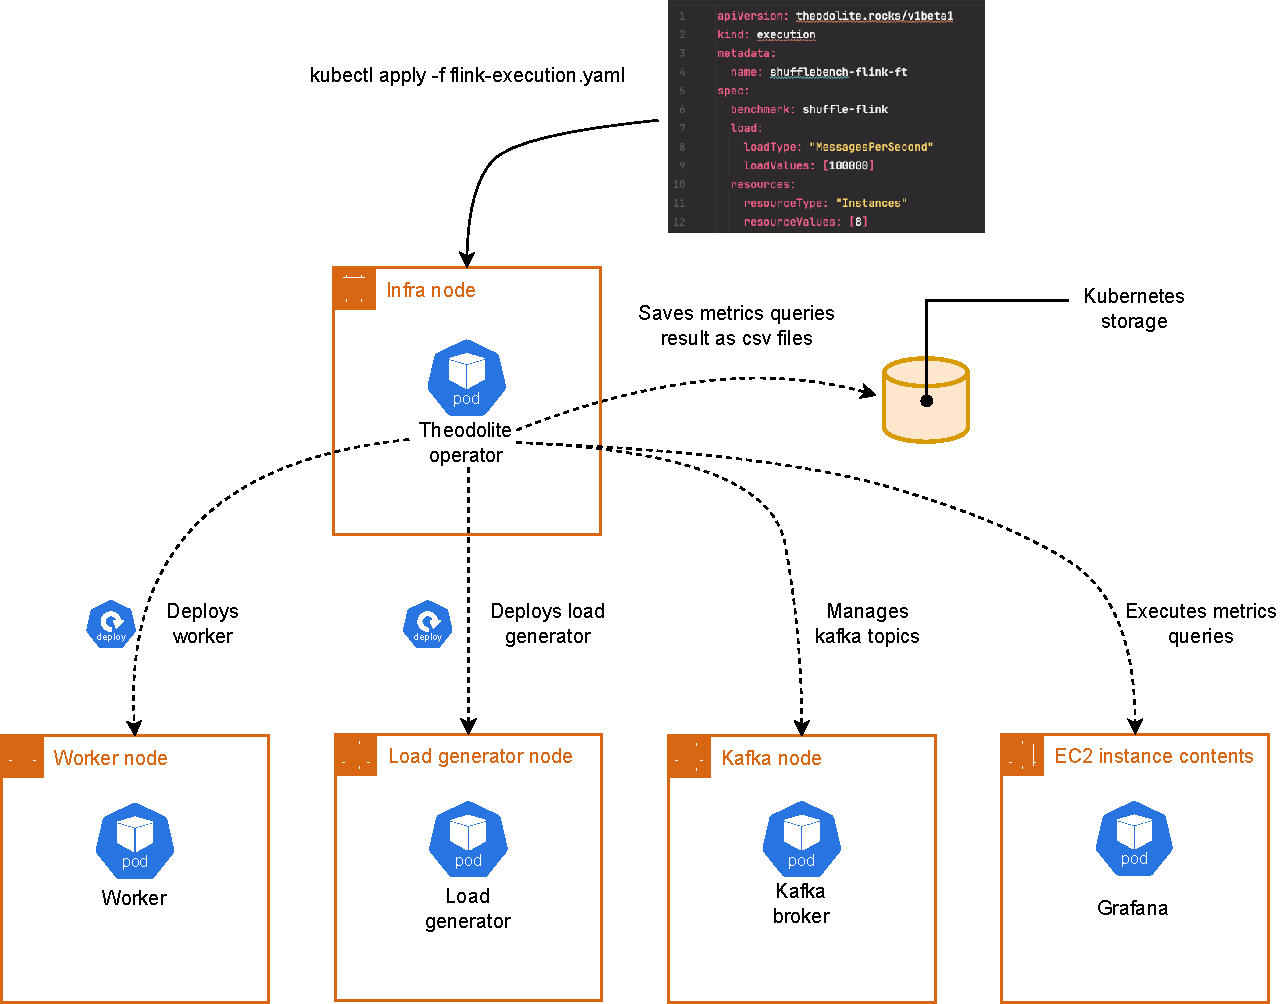
\includegraphics[width=1\textwidth]{figures/theodolite-process}
    \caption{\textit{Theodolite manages deployment and undeployment of load generator and workers during experiment execution.}}
    \label{fig:theodolite-process}
\end{figure}

To run execution with Theodolite, some preconfiguration has to be made.
Theodolite needs to get access to Kubernetes deployment files for Kafka Streams,
Apache Flink.
Deployment for load generator and monitoring tools comes with Theodolite our of the box.
For custom usage, it is possible to override some deployment configurations.
Apache Flink and Kafka Streams deployment files have to be stored in Kubernetes as config maps \cite{kubernetesConfigMap}.
After each benchmark execution, Theodolite automatically undeploys load generator and workers.


\section{Chaos Engineering with Chaos Mesh}\label{sec:chaos-mesh}

\begin{figure}[ht]
    \centering
    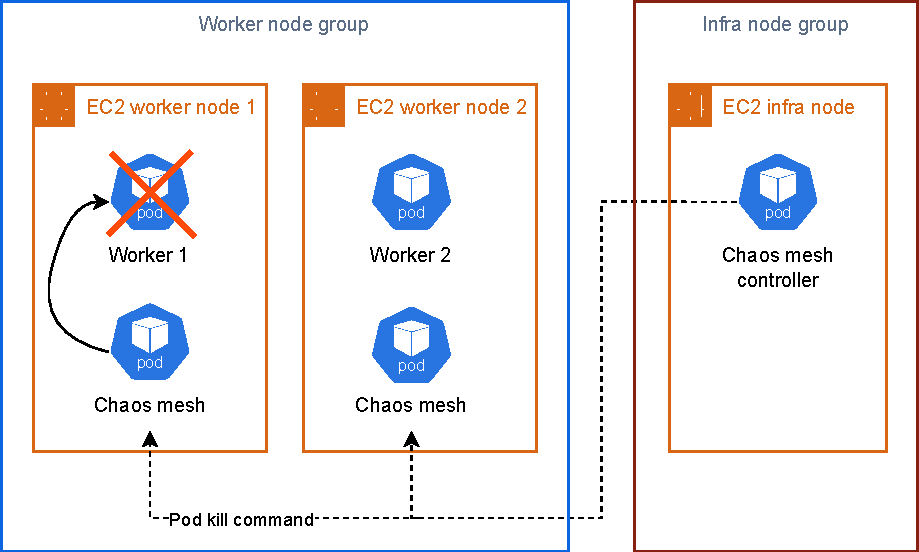
\includegraphics[width=1\textwidth]{figures/mesh-pod-kill}
    \caption{\textit{Example of Chaps Mesh periodic Pod kill. Chaos Mesh controller selects Chas Mesh daemon to
    and sends a message to kill the worker.}}
    \label{fig:chaos-mesh-kill}
\end{figure}

Chaos Mesh \cite{chaosMesh} is a tool used in the Kubernetes environment to simulate
different kinds of failures.
In this case study it is used to kill worker node by using pod selector.
Each deployed worked has its own label, for example, type:worker.
For all experiments, Chaos Mesh is configured to kill worker pods every 3 minutes.
An example use of Chaos Mesh in this case study is depicted on Figure \ref{fig:chaos-mesh-kill}.
Chaos Mesh installs Chaos daemon on each worker node, such that has
Chas Mesh contoller has access to worker pods for failure simulation.
However, Kubernetes quite fast redeploys killed worker replicas, but this time is more than enough
to find valuable metrics about how the system would behave.
For example, Kafka Streams and Apache Flink use different re-partitions algorithms to
handle load balancing.
Depending on re-partitions strategies, this case study can show this difference by measurement
a stare recovery time.

\section{Experiment Setup}\label{sec:experiment-setup}
This section describing experiment execution steps to show how to deploy benchmarks setup and
get benchmarks as csv files from scratch.

\subsection{Prerequisite}\label{subsec:prerequisite}
To get started with benchmarks execution, some steps need to be finished first.

\begin{description}
    \item[Prototype compilation] Build prototypes source code.
    \item[Docker images] Once code is compiled, Docker images need to be built and deployed
    to ECR \cite{awsECR} service which is AWS image storage.
    \item[Kubernetes Deployment configuration] Configure deployment configuration files for Apache Flink
    and Kafka Streams prototypes.
\end{description}

Built Docker images and configured Kubernetes deployment files are
prerequisite to get started with Theodolite and EKS deployment.

\subsection{EKS Cluster}\label{subsec:eks-cluster}
Execute command with eksctl tool EKS cluster configuration in cluster.yaml  \ref{lst:eks-cluster}.

\begin{lstlisting}[label={lst:eks-cluster}]
    eksctl create cluster -f cluster.yaml
\end{lstlisting}

Once the cluster is created, EBS and EFS network storage have to be configured.
For EFS the following installation guide needs to be done first \cite{awsEfsCsi}.
The Next step is applying EBS and EFS storage configuration \ref{lst:eks-storage}.

\begin{lstlisting}[label={lst:eks-storage}]
    kubectl apply -f kafka-storage-class.yaml
    kubectl apply -f flink-storage-class.yaml
\end{lstlisting}


\subsection{Theodolite Configuration}\label{subsec:theodolite-isntllation}
Prerequisite is values.yaml with defined node selector for EKS node groups,
it should not be installed to worker and load generator nodes.

\begin{lstlisting}[label={lst:theodolite-inst}]
    helm install theodolite theodolite/theodolite -f values.yaml
\end{lstlisting}

These Kubernetes config maps load deployment files to Kubernetes config such that Theodolite
has access to files within Kubernetes.
\begin{lstlisting}[label={lst:config-map}]
    kubectl create configmap --from-file ./shuffle-load-generator/
    kubectl create configmap --from-file ./shuffle-latency-exporter/
    kubectl create configmap --from-file ./shuffle-kstreams/
    kubectl create configmap --from-file ./shuffle-flink/
\end{lstlisting}


These commands tell Theodolite how to access config maps created in a previous step \ref{lst:config-map}.
\begin{lstlisting}[label={lst:config-map-theodo}]
    kubectl apply -f theodolite-benchmark-kstreams.yaml
    kubectl apply -f theodolite-benchmark-flink.yaml
\end{lstlisting}

At this step, deployment configurations should be ready to be used during experiments.


\subsection{Running Experiments}\label{subsec:running-experiments}
To run experiments, Thedolite is listening for execution files to be applied but
kubectl.
Theodolite Kubernetes execution file represents instruction for Theodolite operator
about how to run experiments.
For example, what services to deploy, how log should experiment be running, environmental
variables, how many repeats have to be.
Experiment execution could be described in the following steps:

\begin{description}
    \item[Appy execution config] Once Theodolite operator found the execution config, it's
    starting deploying components which are need to be running only during the experiment execution.
    In this case study, these are: load generator, latency exporter, Kafka Streams or Apache Flink
    workers replicas.
    \item[Running experiment] Based on the execution config, the experiment is running for a certain
    time period, in this case study it's 18 minutes.
    \item[Finishing experiment] Once the execution time has passed, Theodolite operator undeploy,
    deployed services at execution start, executes PromQL queries to get benchmarks from Grafana,
    and saves them as CSV files.
\end{description}

Examples of csv files with recorded benchmarks produced by Theodolite operator.
Each experiment has its own set of benchmarks.

\begin{lstlisting}[label={lst:bench-csv-files}]
    exp3_managerNodesDiskReadMB_2s_1.csv
    exp3_generic_latency_p90_30s_1.csv
    exp3_kafkaBrokerNodesCPUsPercentageUtilization_2s_1.csv
    exp3_workerNodesCPUsPercentageUtilization_2s_1.csv
\end{lstlisting}


%\section{Benchmarks metrics}\label{sec:benchmarks-metrics}
%Benchmarks setup for the case study is exploring the following metrics:
%
%\begin{itemize}
%    \item Average worker nodes CPU utilization.
%    \item Output throughput per broker.
%    \item Output throughput per partition.
%    \item Input throughput per broker.
%    \item Input throughput per partition.
%    \item Input throughput.
%    \item Kafka broker node CPU utilization.
%    \item Kafka broker nodes disc read.
%    \item Kafka broker nodes disc write.
%    \item Kafka broker nodes network received.
%    \item Kafka broker node networks transmitted.
%    \item Kafka input topic lag per partition.
%    \item Kafka laf per repartition.
%    \item Kafka message latency p50.
%    \item Kafka message latency p90.
%    \item Kafka message latency p95.
%    \item Kafka message latency p99.
%    \item All nodes CPU utilization.
%    \item Number of worker replicas.
%    \item Output throughput.
%    \item Pods CPU percentage utilization.
%    \item Pods CPU total utilization.
%    \item Pods IO memory ped pod.
%    \item Pods network received.
%    \item Pods network transmit.
%    \item Worker nodes CPU utilization.
%    \item Worker nodes disk read.
%    \item Worker nodes disk write.
%    \item Worked nodes network received.
%    \item Worker nodes network transmit.
%    \item Kafka consumer group lag trend.
%\end{itemize}
%
%Based on the metrics above, the case study is trying to make a
%conclusion about performance difference between Kafka Streams and Apache Flink
%in case of fault tolerance with a state recovery.

%\subsubsection{Load Generator}
%The load generator is only designed to generate a stream of Kafka messages, where
%each message is a random byte array of 1KB size.
%The generator is based on a simple spring boot app, where the load of messages is
%generated with ScheduledThreadPoolExecutor of 4 threads.
%A nature of the mode generator requires more cpus rather than a disc space.
%
%The node group of the generator consists only of a single node of a type m6i.xlarge.
%This node is efficient enough to generate 200K MPS and even much more.
%
%\subsubsection{Kafka Streams}
%Kafka Streams as well as the load generator is based on Spring Boot framework since it is
%the mose popular and common framework for running Java applications and provides out of the box
%support for Kafka Streams.
%It's important to have as fewer configurations as possible to simply run and Deploy Kafka Steams
%instance.
%Kafka Steams node groups consists of m6in.xlarge type nodes.
%
%\subsubsection{Apache Flink}
%Apache Flink requires a different approach for node groups comparing to Kafka Streams since
%it has a different architecture and includes additional components to run and manage streaming
%jobs.
%For this benchmarking experiments two separate node groups were used.
%The first one of for Flink job manager and the second one is for Flink task managers which
%are workers.
%Flink job managers require much less resources since they are intended to control task managers.
%For these experiments for task managers was chosen a node groups of type t3.medium.
%For task managers was chosen a more performant node type m6in.xlarge.
%The same type was used for Kafka Streams to compare a resource consumption for two solutions.
%
%However, these experiments required additional component for the Flink cluster which is
%Flink Kubernetes Operator.
%It is open source and open source solution to dramatically simplify a Flink cluster management.
%For experiments, it was running withing the monitoring node group since it doesn't consume
%many resources.
%
%\subsubsection{Monitoring}
%The following group was used as a default node group for any other services, like Prometheus,
%Grafana, Prometheus Operator, Flink Operator.
%Monitor node groups consists of two nodes of type t3.medium.
%
%\subsection{Infrastructure as Code}\label{subsec:infrastructure-as-code}
%With such complex cloud setup, it's simple not possible to create and such
%complex infrastructure and fortunately there are available tools for such use cases.
%The main tools which were used for experiments are \textbf{Helm} and \textbf{kubectl}
%
%\begin{description}
%    \item[Helm] is a tool which manages packages for Kubernetes cluster, it allows to create,
%    update and deleted Kubernetes resources.
%    \item[kubectl] is a cli tools which also allows to manage resources, but not as a package but
%    rather each resource separately.
%\end{description}
%
%For experiments, were create all required Kubernetes resources which makes deployment
%quite fast and efficient.
%
%For each experiment there's a set of Kubernetes resource files which is used
%for a specific benchmark.
%It makes deployment easier and less error-prone, however it might bring
%too much boilerplate code.



%\section{Implementation Details}\label{sec:implementation-details}
%This section covers use case implementation with Kafka Streams and Apache Flink.
%The source code for Apache Flink and Kafka Streams is Java Gradle based project,
%where gradle version is 8.5 and jar were build with Java 11 and Java 21.
%Both builds were deployed to Amazon ECR, such that once deployed Docker images
%are reusable and not required to be built for each experiment separately.
%The core image built platform is Docker.
%In order to deploy build images two cli tools were used.
%
%\begin{description}
%    \item[Docker cli] is a tool which help to build Docker images with the app and deploy them
%    to Kubernetes cluster.
%    Quite important to use a correct platform, for experiment were chosen Linux distros, for
%    this reason the following build parameter was used --platform=linux/amd64.
%    Moreover, docker cli provide aws login system which knows how to deploy build images directly to
%    Amazon ECR.
%    \item[aws cli] is a cli which provides API to work with AWS resources, docker cli
%    is integrated with the aws cli quite well.
%\end{description}


%\subsection{Rule Based Matcher}\label{subsec:rule-matcher}
%
%\begin{figure}[H]
%    \centering
%    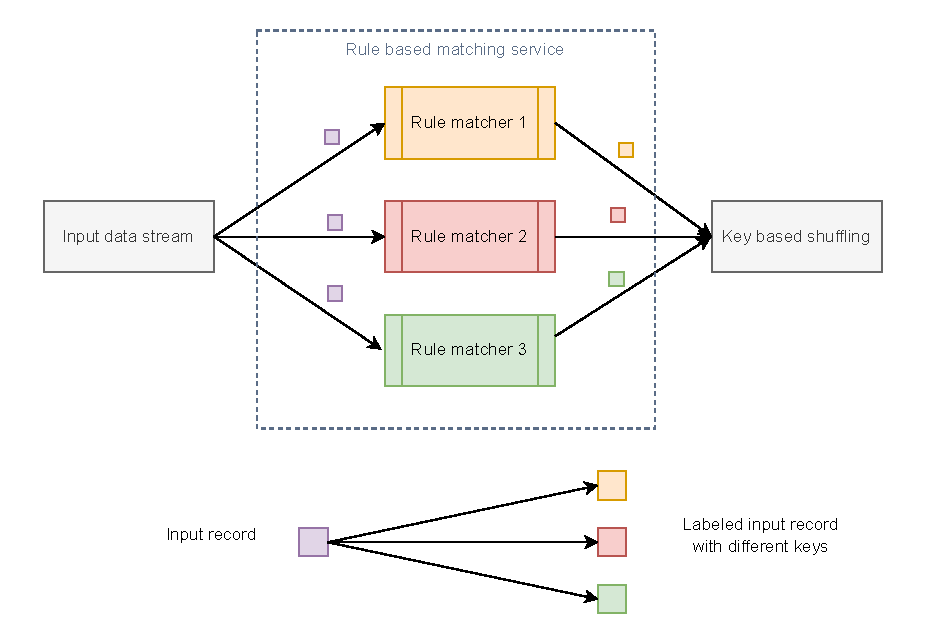
\includegraphics[width=1\textwidth]{figures/rule-matcher}
%    \caption{\textit{Rule based matcher.}}
%    \label{fig:rule-matcher}
%\end{figure}
%
%This is the core component of streaming pipeline for the use case.
%It could be considered as a black box which provides a single api method to match
%incoming bytearray record.
%Its logic could be described using diagram above ~\ref{fig:rule-matcher}.
%
%The matched has a single method interface for byte array record which
%can based on defined rules is able to matched with them.
%All matched rules get shuffled by name which makes to distributed
%further processing among all replicas.
%The main parameters of the matcher are selectivity and number of rules.
%
%\begin{description}
%    \item[Matching Rule] is a rule which has a selectivity property to be matched with a byte array record.
%    \item[Selectivity] is a value with a floating point which defined a probability witch record can be
%    matched.
%\end{description}
%
%For example, if the matcher has 10000 rules, with selectivity of 0.00002, then a probability with
%which it will be matched with incoming record is 0.00002\%.
%These values could be different depending on a system simulation.
%The matcher is a prototype which is supposed to simulate a real service.
%Since the rule matched is not a focus of the research, it is more than enough to use
%a prototype.

%\subsection{Kafka Streams Implementation}\label{subsec:kafka-streams-implementation}
%
%\begin{figure}[H]
%    \centering
%    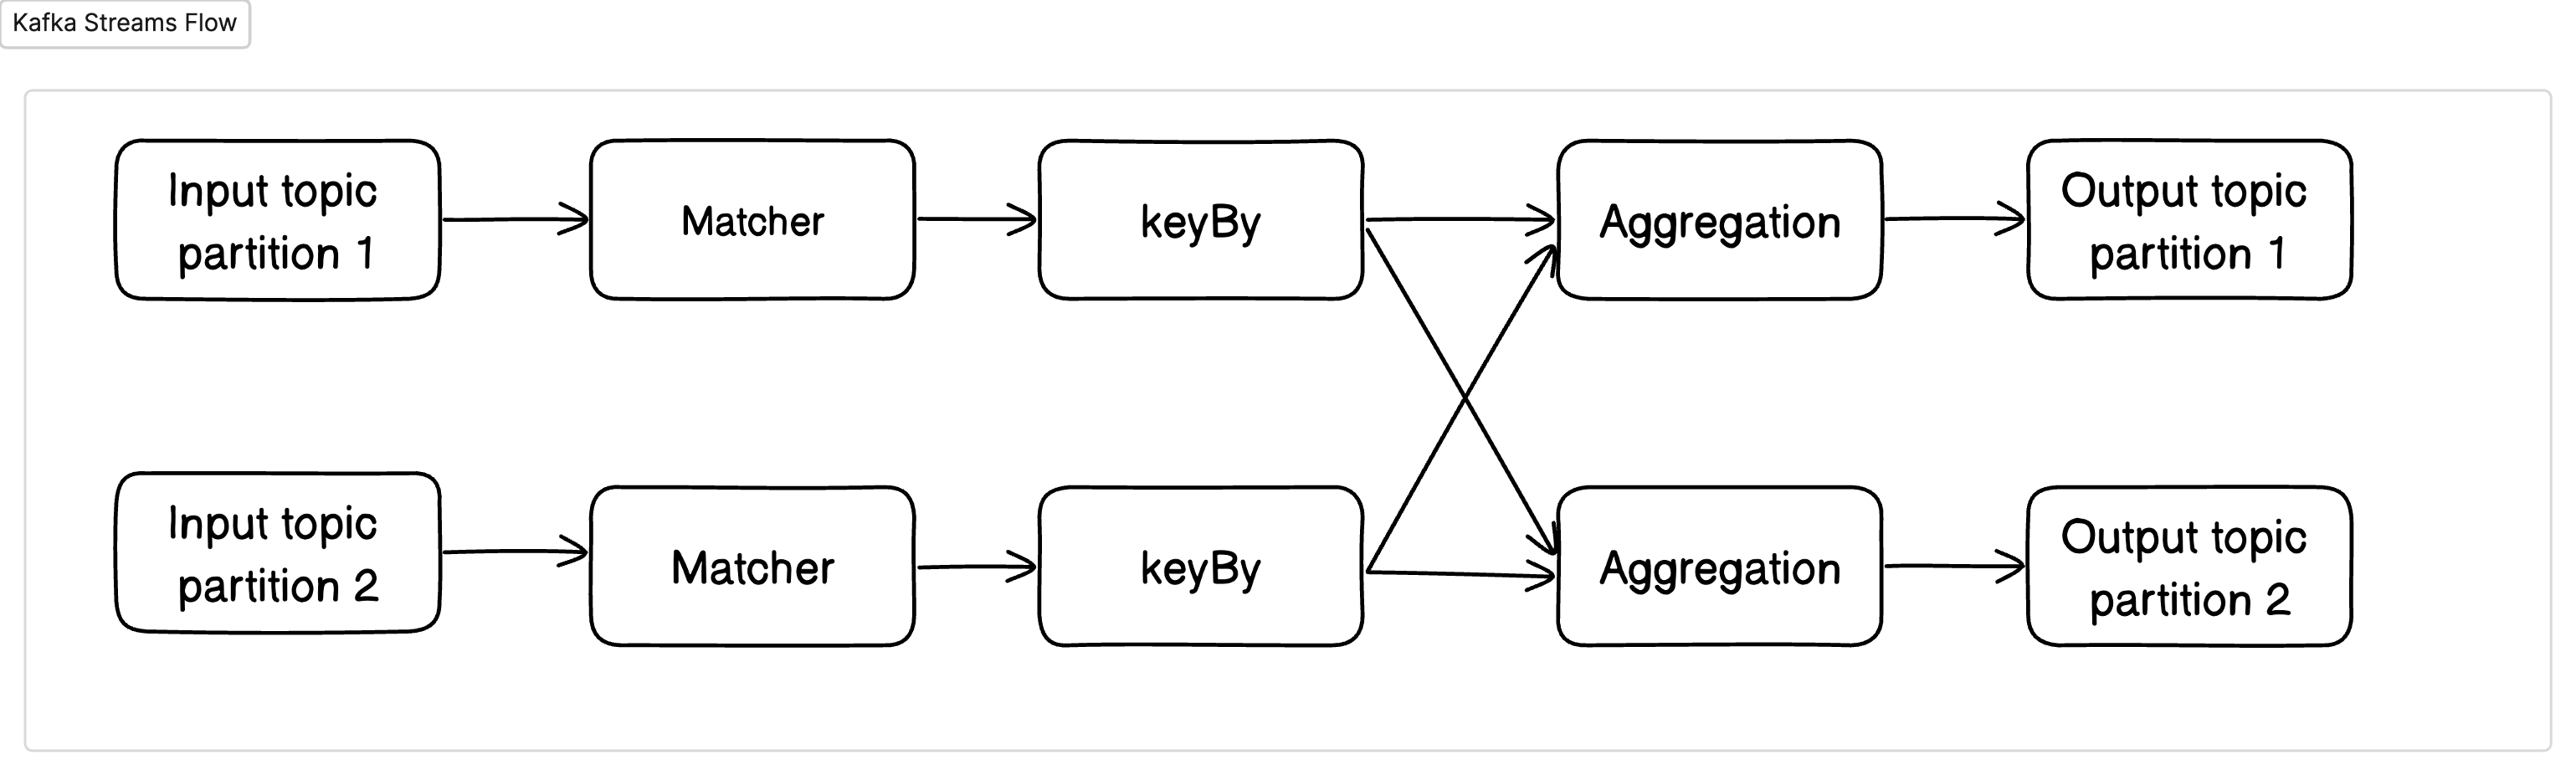
\includegraphics[width=1\textwidth]{figures/k-streams-shuffle}
%    \caption{\textit{Kafka Streams flow.}}
%    \label{fig:k-stream-shufle}
%\end{figure}
%
%Kafka Streams flow is presented on the figure above ~\ref{fig:k-stream-shufle}.
%For the experiments Kafka Streams use default configurations with Kafka
%commit time period of 30 seconds.
%
%
%\subsection{Flink Implementation}\label{subsec:flink-implementation}
%
%\begin{figure}[H]
%    \centering
%    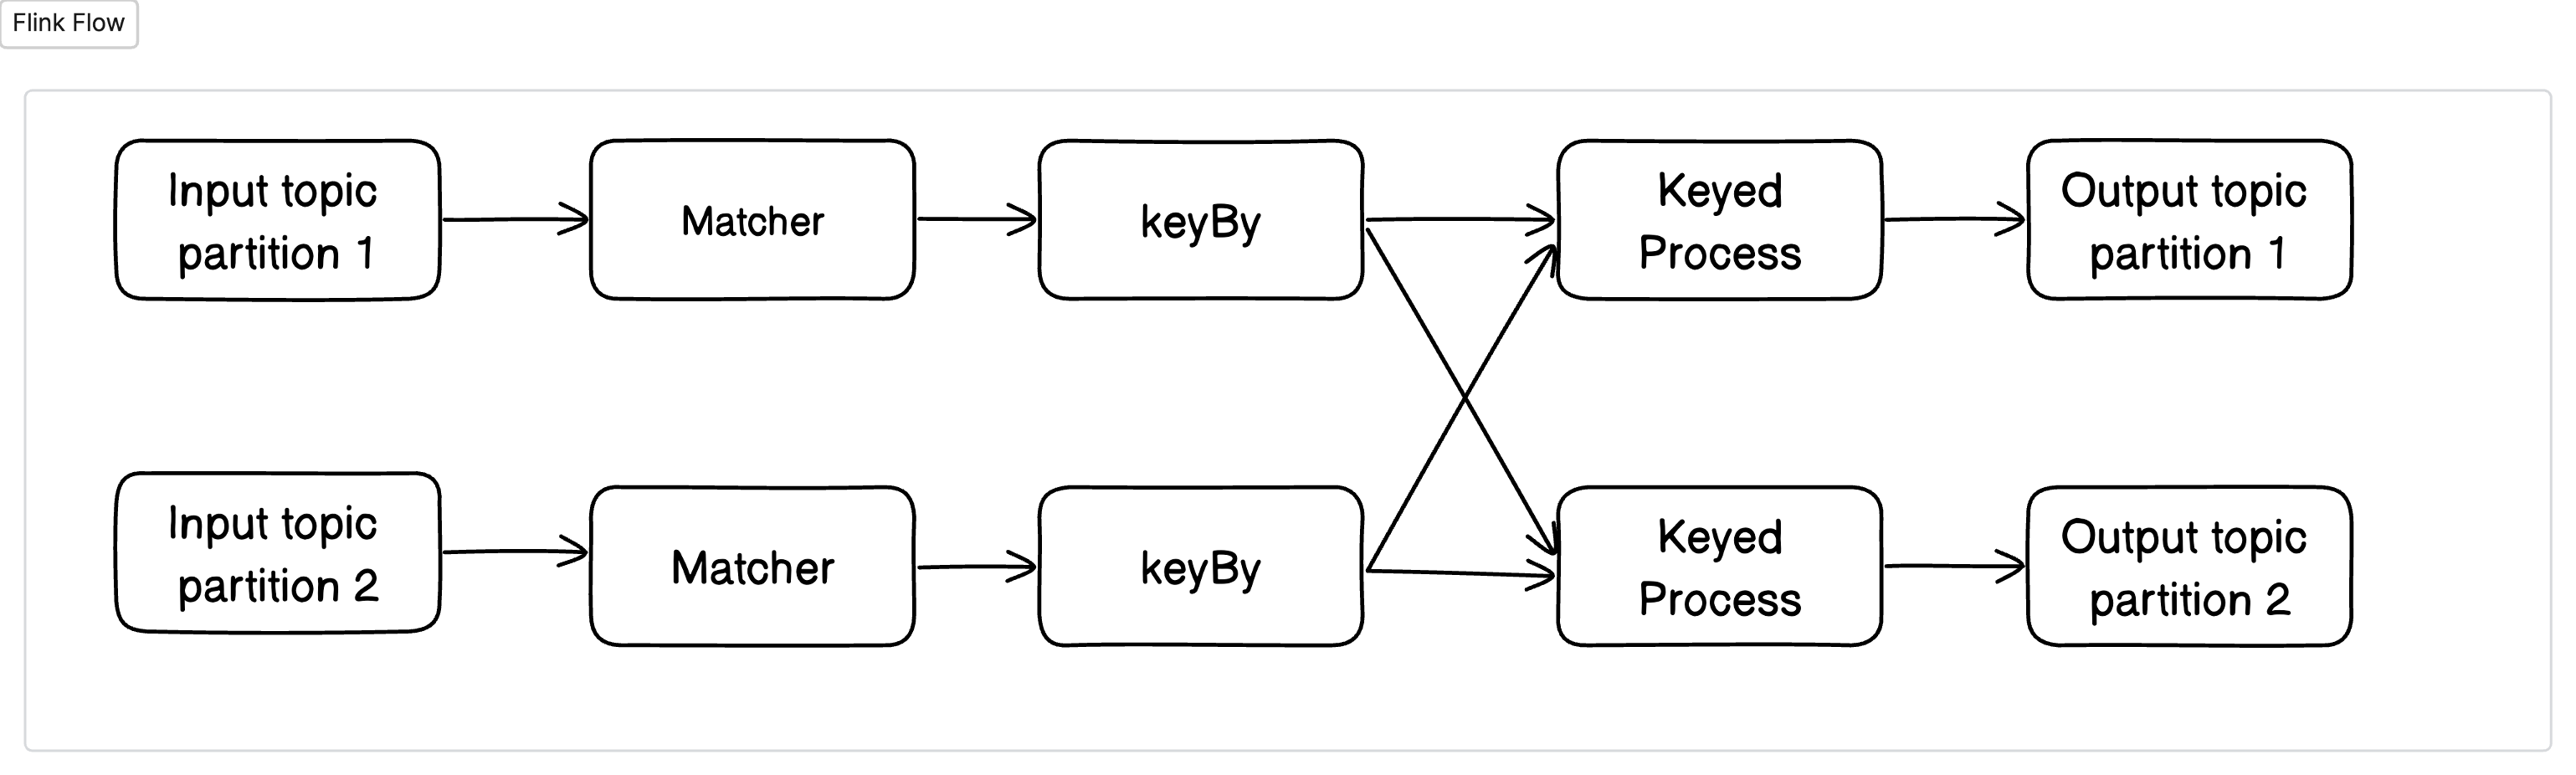
\includegraphics[width=1\textwidth]{figures/flink-shuffle}
%    \caption{\textit{Flink flow.}}
%    \label{fig:flink-shuffle}
%\end{figure}
%
%Flink is using keyed process which also type of aggregation but with a little
%bi different behaviour.
%Flink implementation uses checkpoints, which are get saved every 30 seconds
%to Amazon S3 storage.
%It was done to get the Kafka commit interval like in
%Kafka Streams implementation.
%The same commit interval helps to compare a performance difference.
%
%However, experiments with Flink require to install to EKS cluster additional
%dependencies which are need to manager Flink cluster.
%These tools are: cert-manager for Kubernetes cluster, Flink Kubernetes Operator,
%RBAC roles and permission for Flink Operator which must be allowed to
%deploy Flink task managers and job managers.
%
%



\chapter{Model and its implementation}\label{ch:impl}
This chat provides an overview over a use case implementation.

\chapter{Benchmarks}\label{ch:impl-bench}
\input{chapters/benchmarking-implementatin}

\chapter{Summary}\label{ch:summary}
\input{chapters/summary}


\pagebreak
\phantomsection
\addcontentsline{toc}{chapter}{References}
\printbibliography[title=References]

\pagebreak
\phantomsection
\appendix
% \addcontentsline{toc}{chapter}{Appendices}
% \chapter*{Appendices}
\renewcommand{\thechapter}{\arabic{chapter}}

% License
\newcommand{\licenseFootnote}{The non-exclusive licence is not valid during the validity of access restriction indicated in the student's application for restriction on access to the graduation thesis that has been signed by the school's dean, except in case of the university's right to reproduce the thesis for preservation purposes only. If a graduation thesis is based on the joint creative activity of two or more persons and the co-author(s) has/have not granted, by the set deadline, the student defending his/her graduation thesis consent to reproduce and publish the graduation thesis in compliance with clauses 1.1 and 1.2 of the non-exclusive licence, the non-exclusive license shall not be valid for the period.}
\addcontentsline{toc}{chapter}{Appendix 1 -- Non-Exclusive License for Reproduction and Publication of a Graduation Thesis}\label{chapter:license}
{\let\clearpage\relax\chapter*{Appendix 1 -- Non-Exclusive License for Reproduction and Publication of a Graduation Thesis\footnote{\licenseFootnote}}}
% Generates the list of supervisors. Do not edit
\newcommand{\supervisorList}[1]
{
  \ifthenelse{\equal{#1}{[Co-Supervisor's Name]}}{\mbox{\supervisor}}{\mbox{\supervisor}~and \mbox{\cosupervisor}}
}

% The license should be automatically filled, please double check that everything is fine before submitting
I \authorName

\begin{enumerate}[label*=\arabic*.]
    \item Grant Tallinn University of Technology free licence (non-exclusive licence) for my thesis ``\doctitle'', supervised by\supervisorList{\cosupervisor}
    \begin{enumerate}[label*=\arabic*.]
        \item to be reproduced for the purposes of preservation and electronic publication of the
graduation thesis, incl. to be entered in the digital collection of the library of Tallinn
University of Technology until expiry of the term of copyright;
        \item to be published via the web of Tallinn University of Technology, incl. to be entered in the digital collection of the library of Tallinn University of Technology until expiry of
the term of copyright.
    \end{enumerate}
    \item I am aware that the author also retains the rights specified in clause 1 of the non-exclusive licence.
    \item I confirm that granting the non-exclusive licence does not infringe other persons' intellectual property rights, the rights arising from the Personal Data Protection Act or rights arising from other legislation.
\end{enumerate}

% Defaults to current date. If you want a specific date, replace \signaturedate with hardcoded value
\signatureDate


% Other appendices
% NOTE: Appendix 1 is always the non-exclusive license.
% Therefore, your appendices need to start from 2.

%\clearpage
%\phantomsection
%\addcontentsline{toc}{chapter}{Appendix 2 -- Something}\label{chapter:appendix-something}
%\chapter*{Appendix 2 - Something}
%\begin{lstlisting}[frame=single, basicstyle=\small]
<!DOCTYPE html>
<html>
<body>

<h1>Example Title</h1>

<p>Some text here</p>

</body>
</html>
\end{lstlisting}

%
%\clearpage
%\phantomsection
%\addcontentsline{toc}{chapter}{Appendix 3 -- Something Else}\label{chapter:appendix-something-else}
%\chapter*{Appendix 3 -- Something Else}
%\textbf{Pythagorean theorem}
\begin{equation}
x^n + y^n = z^n
\end{equation}

\textbf{Normal distribution}%
\begin{equation}
P(x) = \frac{1}{{\sigma \sqrt {2\pi } }}e^{{{ - \left( {x - \mu } \right)^2 } \mathord{\left/ {\vphantom {{ - \left( {x - \mu } \right)^2 } {2\sigma ^2 }}} \right. \kern-\nulldelimiterspace} {2\sigma ^2 }}}
\end{equation}


\end{document}